\part{Real fluids}


\chapter{Navier-Stokes equations}

\section{Kinematics of a particle}
Let us focus again on a fluid particle, as we did on \ref{sec:}, but
now focusing on how the particle itself distorts as a consequence of a
velocity field.

All possible distorsions of a particle will be a combination of the
following:
\begin{enumerate}
 \item Translation
 \item Rotation
 \item Shear
 \item Dilation
\end{enumerate}

A translation is just the motion of its center of mass from one place
to another, and for a small time is given simply by $\bfu dt$. The
other motions are more complicated, since they involve spatial
derivatives of the velocity. They must: for a constant velocity field
translation is the only mode that occurs.

\subsubsection{Rotation}

We will refer to particle in figure \ref{fig:}, with vertices A, B,
and C. Vertex D plays no role --- also, it is sufficient to focus on
the face that is portrait, even if the shape of a particle is supposed
to be a cube. It is straightfoward to include the other faces, as we
will see.

After a small time $d$ the particle has distorted, so that the
vertices are now at positions A', B', C', and D'.

\begin{figure}
  \centering
  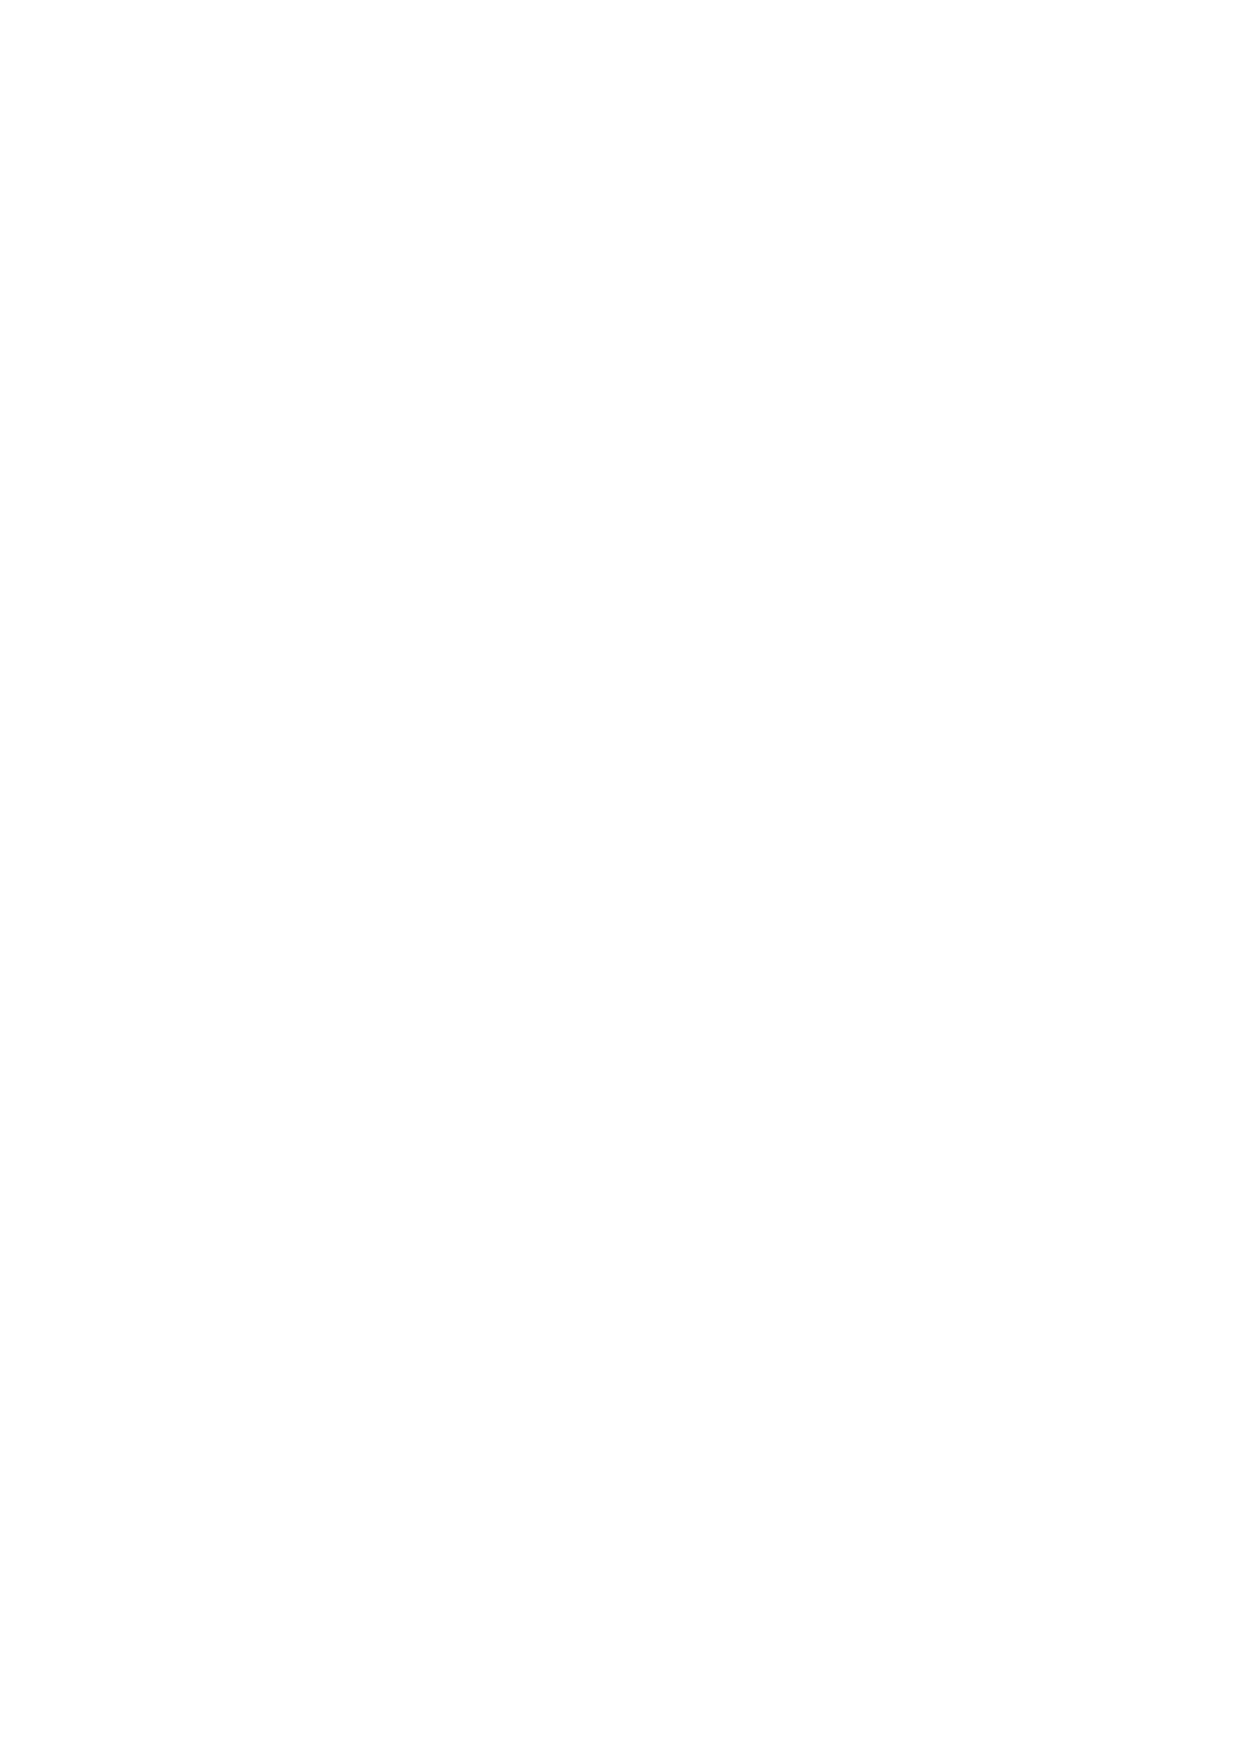
\includegraphics[width=0.4\linewidth]{figures/particle0}
  \caption{\label{fig:particle0}}
\end{figure}



Let us call $\alpha$ the angle between the $x$ axis and the A'-B'
edge, with the usual counter-clockwise convention as
positive. Similarly, $\beta$ is the angle between the A'-C' edge and
the $y$ axis, with the same convention. It is obvious that a net
rotation takes place if e.g. both angles are positive. If, on the
other hand, they are equal in magnitude but differ in sign, no
rotation takes place. This makes it reasonable to define the
rotation as the average of both angles:
\[
d\Omega_z = \frac12
\left(
        \alpha + \beta
\right) .
\]

Now, angle $\alpha$ will always be very small as $dt$ gets very
tiny. Hence, we may approximate it by its tangent:
\[
\alpha \approx \frac{d\ell}{dx'}
\]



\begin{figure}
  \centering
  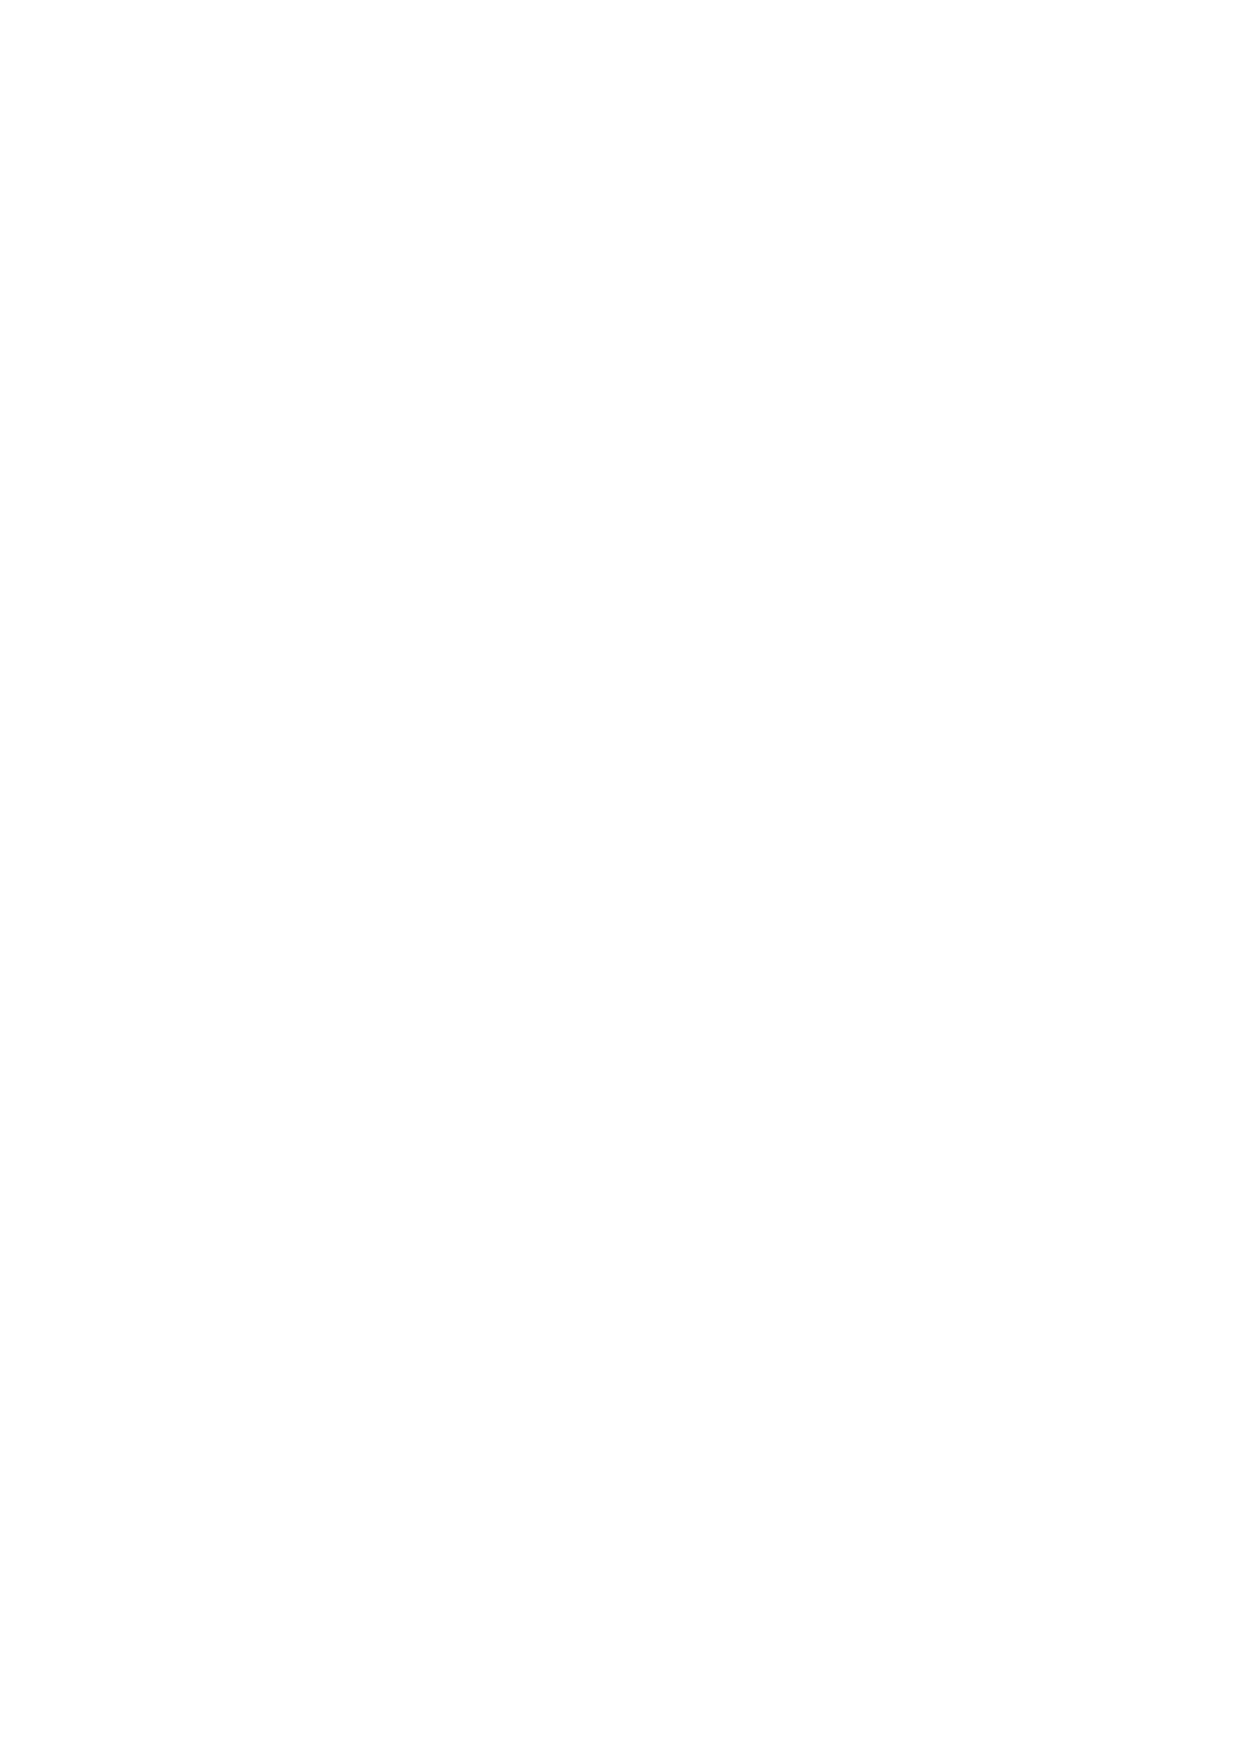
\includegraphics[width=0.4\linewidth]{figures/particle1}
  \caption{\label{fig:particle1}}
\end{figure}

For a small time, we have the following:
\[
dx'=x(B')-x(A') \approx
(dx+v_x(B) dt) - v_x(A) dt \approx
dx+
\left(
v_x(A) +
\frac{\partial v_x}{\partial x} dx
\right ) dt - v_x(A) dt = dx + \frac{\partial v_x}{\partial x} dx dt ,
\]
where we have taken the origin to coincide with the position of A. The
partial derivative is supposed to be evaluated at A, but in the limit
as $dx$ goes to zero it is just ``at the particle''. Similarly, the opposing
side is:
\[ 
d\ell = y(B')-y(B) \approx
v_y(B) dt \approx
\left(
v_y(A) +
\frac{\partial v_y}{\partial x} dx
\right ) dt = \frac{\partial v_y}{\partial x} dx dt ,
\].

Therefore, to first order in $dt$:
\[
\alpha \approx \frac{\partial v_y}{\partial x}  dt .
\]
In other words, the rate of change of the angle is
\[
\frac{d \alpha}{dt} = \frac{\partial v_y}{\partial x}  .
\]
Notice the cross derivative: what is relevant is the change of the
vertical component of the velocity with the horizontal coordinate.

A similar calculation for the other angle reveals
\[
\frac{d \beta}{dt} = - \frac{\partial v_x}{\partial y}  .
\]

Taking all
\[
\frac{d\Omega_z}{dt} = \frac12
\left(
  \frac{\partial v_y}{\partial x}  -
  \frac{\partial v_x}{\partial y}
\right) .
\]

This may sound familiar to the reader, since the curl in Cartesian
coordinates has a $z$ component with exactly the same expression, but
the factor of $1/2$. This analysis may be carried out for
rotations about the other two Cartesian axes, with the end result that
\[
 \frac{d \bm{\Omega} }{dt} = \frac12 \vort .
\]

The curl is therefore twice the rate of rotation of a fluid particle.


An example

Let us consider a uniform circular motion about the origin:
\[
\bfr =
\begin{cases}
&x=r \cos(\omega_0 t) \\
&y=r \sin(\omega_0 t) .
\end{cases}
\]
The velocity field is
\[
\bfu =
\begin{cases}
&u_x= -r \omega_0 \sin(\omega_0 t) = -\omega_0 y \\
&u_y=  r \omega_0 \cos(\omega_0 t) =  \omega_0 x.
\end{cases}
\]

If we compute the curl of this field, its only component is the $z$ one:
\[
\omega_z= \left(
  \frac{\partial (\omega_0  x)}{\partial x}  -
  \frac{\partial (- \omega_0 y) }{\partial y}
\right) =  2 \omega_0 . 
\]

Therefore, the curl indeed is twice the angular velocity.


\subsubsection{Strain}




\section{Stress tensor}

Let us return again to our particle in order to analyze its movement
when stress forces are applied onto its walls. The pressure force may
be consider a special case of the latter, but stress forces may also
have a shear component.

Thus, the horizontal force will be given by, in part, by the
contributions due to the walls at the left, back, and bottom
\begin{equation}
  \label{eq:wall_shear_stress}
  \left. dF_x \right|_\text{l,bk,bm} =
  % - p         dy\, dz
    \tau_{xx} dy\, dz
    \tau_{yx} dx\, dz
    \tau_{zx} dx\, dy .
\end{equation}
%
The compression stress $\tau_{xx}$ is therefore quite similar to the
pressure (see (Eq \ref{eq:}), and in fact will be seen to include a
$-p$ term. The minus sign appears because normal stresses are
historically defined as positive if pointing outside the particle
(i.e. in the direction of the normal vector).
%
%where we include not only the pressure force, as before 
%and a compression stress $\tau_{xx}$ quite similar to it,
In addittion, two shear stress forces appear. One of them, $\tau_{yx}
dx\, dz$ is the horizontal shear force on the back wall ($dx\, dz$
actually equals $dx\, dy$, but it is clearer to write it this
way). Similarly, $\tau_{zx} dx\, dy $ is the horizontal stress force
at the bottom wall.

Notice the convention for labeling: $\tau_{ij}$ is the stress in the
$j$ direction on a face normal to axis $i$. I.e. the left face has the
same convention as the right one, the back as the front, the top as
the bottom.

%First, the normal stress is
%$\tau_{xx} \parallel \bfn $. From it,
%$\tau_{xy} \parallel \bfe_z\times \tau_{xx} $,
%$\tau_{xz} \parallel \tau_{xx} \times \bfe_y $, respecting the
%$(x,y,z)$ cyclic order. A quick way to realize this is by considering
%the top face, on which these three directions coincide with the
%Cartesian axes. The directions on other faces are found by rotating
%these directions accordingly. The right hand may be used for this
%purpose.

To get the whole horizontal force, the contributions from the other
three walls must be considered:
\[
\left. dF_x \right|_\text{r,ft,up} =
%- p         dy\, dz
  \tau_{xx}(x+dx,y   ,z   )  dy\, dz +
  \tau_{yx}(x   ,y+dy,z   )  dx\, dz +
  \tau_{zx}(x   ,y   ,z+dz)  dx\, dy .
\]
%This time, the sign convention is positive.

To get the total horizontal force due to stresses, the two contributions
must be substracted:
\[
dF_x =
\left( \tau_{xx}(x+dx,y   ,z   ) - \tau_{xx} \right) dy\, dz +
\left( \tau_{yx}(x+dx,y   ,z   ) - \tau_{yx} \right)  dx\, dz +
\left( \tau_{zx}(x+dx,y   ,z   ) - \tau_{zx} \right) dx\, dy .
\]
Notice that the substraction is in order: if the stresses are the same
on those faces, the resultant force will then be zero (those forces
may exert a net torque, but not a force).  In general, they will be
different on those faces, as as been made explitic on their arguments.

The choice is such that an variation in a given direction is assigned
a positive sign. This affects later results, in particular the fact
that the pressure appears with a negative sign.

Expanding in Taylor series, we get the following net horizontal force:
\[
 dF_x  =
%-\frac{\partial p      }{\partial x}  dx\, dy\, dz
% +
 \left(\frac{\partial\tau_{xx}}{\partial x}  dx\right)\, dy\, dz
+\left(\frac{\partial\tau_{yx}}{\partial y}  dy\right)\, dx\, dz
+\left(\frac{\partial\tau_{zx}}{\partial z}  dz\right)\, dx\, dy .
\]

The volumetric horizontal force is then,
\[
f_x  =
%-\frac{\partial p      }{\partial x}
 %+
 \frac{\partial\tau_{xx}}{\partial x}
+\frac{\partial\tau_{yx}}{\partial y}
+\frac{\partial\tau_{zx}}{\partial z} .
\]

With integer notation for Cartesian coordinates:
\[
 df_1  =
%-\frac{\partial p      }{\partial x_1}
 %+
 \sum_{j=1,2,3}
 \frac{\partial\tau_{j1}}{\partial x_j} .
\]


In general, for any component we will have:
\[
 df_i  =
%-\frac{\partial p      }{\partial x_i}
 %+
 \sum_{j=1,2,3}
  \frac{\partial\tau_{ji}}{\partial x_j} .
\]

In order to use vector notation, we have to introduce the
divergence of a tensor:
\[
\nabla \cdot \tau = \sum_{j=1,2,3}
  \frac{\partial}{\partial x_j}  \tau_{ji} ,
\]
 which results in a vector:
\[
 d\bff  =
%-\nabla p
 %+
 \nabla \cdot \tau .
\]
%
The tensor $\tau$ has components $\tau_{ij}$. There is also
the matrix notation, by which
\[
\nabla \cdot \tau = \nabla\tran  \tau ,
\]
where $\nabla\tran$ is a transposed (row) vector operator, multiplying
matrix $\tau$ from the left.

The resulting Navier-Stokes equation is then,
\[
\rho \frac{d\bfu }{dt} = \nabla \cdot \tau   + \rho \bfg .
\]



\subsection{Newtonian fluids}

The previous equation is still too general, and a connection between
stress and strain is still needed. Here we consider the case in which
there is a linear relationship between both, which involves the
coefficient of viscosity.

To begin with, let us consider a simple case in which a fluid is
confined between two planes. One of them moves sideways with a certain
speed $u_0$, while the other is kept fixed. After a certain transient,
some force is needed in order to keep this shearing. The simplest
expression is
\[
F= \mu A \frac{u_0}{L} .
\]
The force is proportional to the area and to the velocity difference
between the planes. It is also inversely proportional to their
separation, $L$ (this fact being the least obvious). Finally, a
constant of proportionality is given by $\mu$, the viscosity
coefficient, or simply ``the viscosity''. This constant may vary with
temperature, density, pressure, but the point with Newtonian fluids is
that it does not vary with the velocity field (or its
derivatives). Later, in section \ref{sec:}, this flow will be solved
as a solution of the Navier-Stokes equations, the Couette flow. There,
it will be shown that the velocity is everywhere in the direction of
the force exerted on the upper plane, let us call it $x$, and varies
linearly between the planes, in the $y$ direction. Therefore, the only
components of the strain rate tensor are $\epsilon_{xy} =
\epsilon_{yx} = u_0 / ( 2 L )$. We therefore have
\[
\tau_{xy} = \mu  \epsilon_{xy} .
\]

With these in mind, let us look for a general relationship between
$\tau$ and $\epsilon$. This is much easier if we go to the principal
strain axes. These are the coordinates on which the strain rate is
diagonal. Such coordinate system always exist, since the strain rate
tensor is symmetric. Notice that in these system strains are not due to
shear, only to dilations.

A simple example would be to consider the flow $u_x = u_0 y / L$
(again, Couette flow). In this case,
\[
\epsilon=
\begin{pmatrix}
  0           &   u_0/(2L)  \\
   u_0/(2L)   &   0
\end{pmatrix} .
\]

It is easy to find the two eigenvalues and associated eigenvectors of
this matrix:
\begin{align*}
  \lambda_1=  u_0/(2L) \qquad &\bfv_1=(1/\sqrt{2}) \begin{pmatrix} 1 &  1 \end{pmatrix}\tran \\
  \lambda_1= -u_0/(2L) \qquad &\bfv_2=(1/\sqrt{2})  \begin{pmatrix} 1 &  -1 \end{pmatrix}\tran \\
\end{align*}
Notice the first eigenvalue correnspond to a dilation along the $x=y$
diagonal, while the second is a compression along the $x=-y$ one.

The diagonal strain rate matrix is then:
\[
\tilde{\epsilon}=
\begin{pmatrix}
  u_0/(2L)   & 0 \\
  0          & - u_0/(2L)
\end{pmatrix} .
\]

It is crucial to realize that the stress tensor is also diagonal in
this coordinate system. Otherwise, a pure dilation in one of the
principal directions would cause a shear stress in some other
direction. This does not mean, however, that the two tensors are
simply proportional. Instead, we may posit, for the top-most element
\[
\tilde{\tau}_{xx}=
- p + 
C_1 \tilde{\epsilon}_{xx} +
C_2 \tilde{\epsilon}_{yy} +
C_3 \tilde{\epsilon}_{y} .
\]
We have added a $-p$ term that has to be there even when there is no
movement. This is needed, since a diagonal stress tensor $\tau=-p\eye$
produces the $-\nabla p$ term of hydrostatics (in Couette flow, $p$ is
constant, and this term is not needed.) The minus sign of $-p$ stems
from the fact that the pressure force points toward the interior of a
particle.

If isotropy is assumed, there should be no distinction between
traverse directions $y$ and $z$. Therefore, $C_2=C_3$, and
\[
\tilde{\tau}_{xx}=
- p + 
C_1 \tilde{\epsilon}_{xx} +
C_2 ( \tilde{\epsilon}_{yy} +  \tilde{\epsilon}_{y}  ) =
- p + 
K \tilde{\epsilon}_{xx} +
C_2 ( \tilde{\epsilon}_{xx} + \tilde{\epsilon}_{yy} +  \tilde{\epsilon}_{y}  ) ,
\]
where the constant $K=C_1-C_2$. Notice the $C_2$ term is the
divergence of the velocity. But, it is also the trace of the strain
tensor, a quantity which is invariant under change of basis. We can
now write:
\[
\tilde{\tau}_{xx}=
- p + C_2 \nabla\cdot \bfu 
K \tilde{\epsilon}_{xx} .
\]

There will be similar expressions for $\tilde{\tau}_{yy}$ and
$\tilde{\tau}_{zz}$, but in them the coefficients must be the same ---
otherwise isotropy will be violated. Taking all together,
\[
\tilde{\tau}=
K \tilde{\epsilon}
+ ( - p + C_2 \nabla\cdot \bfu ) \eye.
\]

Now, we may go back to the original Cartesian system and find
\[
\tau=
K \epsilon
+ ( - p + C_2 \nabla\cdot \bfu ) \eye.
\]
The stress tensor is then also symmetric, a fact that is required in
order the particle be torsion-free (remember the fact that rotations
have no stress associated.)

A comparison with our previous result reveals $K=2\mu$. The constant
$C_2$ is called, in the theory of elasticity ``the second Lam\'e
coefficient'', and receives the symbol $\lambda$ (it is also called
the ``second viscosity coefficient'', $\mu$ being the first.) Then,
\[
\tau=
2 \mu \epsilon + ( - p + \lambda \nabla\cdot \bfu ) \eye.
\]

To make this explicit, this means that diagonal terms have the form
\begin{equation}
  \label{eq:tau_diagonal}
  \tau_{ii}=
  2 \mu \epsilon_{ii}  - p + \lambda \nabla\cdot \bfu ,
\end{equation}
while off-diagonal terms are
\begin{equation}
  \label{eq:tau_off_diagonal}
  \tau_{ij}=  2 \mu \epsilon_{ij} \qquad j \ne i
\end{equation}


(Why not always work in the system of principal axes? The answer is
simple: principal axes vary from one particle to another, since they
are defined by local values of velocity derivatives. The Cartesian
coordinate system, or any such (cylindrical, polar\ldots) is the same
for all particles.)

The off-diagonal terms have a neat expression when the strain rate
tensor is written in term of velocity derivatives:
\[
\tau_{ij}=
\mu
\left(
\frac{\partial u_i}{\partial x_j} +
\frac{\partial u_j}{\partial x_i}
\right)
\]

The diagonal ones, however, are somewhat puzzling:
\[
\tau_{ii}=
- p +
2 \mu \frac{\partial u_i}{\partial x_i}  + \lambda \nabla\cdot \bfu .
\]
The pressure term is natural, but there are two extra dynamical terms.

Let us define a mechanical pressure as minus one-third times the trace
of the stress tensor:
\[
\bar{p}=
-\frac13 \Tr \tau  = 
 p
- \left( \frac23 \mu  + \lambda \right) \nabla\cdot \bfu .
\]

Defining volume pressure
\begin{equation}
  \label{eq:vol_visc_definition}
  \eta:=\frac23 \mu  + \lambda,
\end{equation}
we may write the mechanical pressure as
\[
  \bar{p}=
  p - \eta \nabla\cdot \bfu .
\]

The result is that the mechanical pressure, defined in such a way, is
different from the thermodynamic pressure in an incompressible fluid.
There are several ways out of this puzzling result. One of them is to
assume simply that the fluid is incompressible. This is of course
entirely correct, but would limit the applicability of the theory to
incompressible problems.

Another approach is to boldly assume $( 2/3 ) \mu+\lambda=0$. This
step was taken by Stokes, and defines a ``Stokesian fluid''. On the
other hand, there is no clear evidence of a real fluid that may
satisfy such a relationship. Indeed, the few measures of $\lambda$
have show positive values (while $\mu$, as should be clear, is always
positive). We should then keep in mind that in some flows when
compressibility is important, mechanical pressure may differ from
thermodynamical one. One such example is the attenuation of sound
waves, explained in Section \ref{sec:sound_waves_att}.

The Navier-Stokes equation for Newtonian liquids is finally:
\begin{equation}
  \label{eq:NS_Newtonian}
  \rho \frac{d\bfu }{dt} =
  - \nabla p +
  2 \nabla \cdot ( \mu \epsilon)
  + \nabla [ \lambda ( \divu ) ]
  + \rho \bfg .
\end{equation}


\subsubsection{Pure shear and compression}

Recalling the definition of the strain tensor $\epsilon$
in Eq. \ref{eq:epsilon_as_grad_u}, the viscous force may be written as
\begin{equation*}
  \bff_\mathrm{v}=
  \nabla \cdot \left[ \mu  \left( \nabla\bfu + \nabla\bfu\tran \right) \right] +
  \nabla \cdot \left[ \lambda (\divu) \eye \right] ,
\end{equation*}
where $\nabla \cdot \left[ A \eye \right] $ is just another way to
write $\nabla A$, for any scalar field $A$.


If the volume viscosity of Eq. \ref{eq:vol_visc_definition} is
introduced, the equation may be rearranged to read
\begin{equation}
  \label{eq:pure_stress_pure_compression}
  \bff_\mathrm{v}=
  \nabla \cdot \left[ \mu  \left(
      \nabla\bfu + \nabla\bfu\tran  - \frac23 (\divu)  \eye
    \right)
  \right] +
  \nabla \cdot \left[ \eta (\divu) \eye \right] .
\end{equation}
This expression is rather elegant, since the term multiplied by $\mu$
describes pure shear flow, with no compression effects, and the term
with $\eta$, pure compression.

This is easily demonstrated, since
\[
  \Tr  \nabla\bfu = \divu \qquad\implies\qquad \Tr \left( \nabla\bfu -\frac13 (\divu) \eye \right) = 0 .
\]
The same goes for $ \nabla\bfu\tran$, hence the $2/3$ factor.


\subsection{Particular instances}

We here consider instancies in which Eq. \ref{eq:NS_Newtonian} for
Newtonian liquid is further simplified.


\subsubsection{Athermal case}

It may happen that the viscosity coefficients do not vary, when the
variations on the other fields are not too great. In particular,
viscosity depends on temperature quite strongly, as is evident when
heating up oil. The temperature has its own equation, to be explained
in the next chapter. In this case, Eq. \ref{eq:NS_Newtonian} may be
written as
\begin{equation*}
  \rho \frac{d\bfu }{dt} =
  - \nabla p +
   2 \mu \nabla \cdot  \epsilon
  + \lambda \nabla ( \divu ) )
  + \rho \bfg .
\end{equation*}

Now, $\nabla \cdot  \nabla\bfu = \nabla^2 \bfu$, as can be demonstrated
since the $i$-th component of the resulting vector is
\[
(\nabla \cdot \nabla\bfu )_i =
\sum_{j=1,2,3} 
\frac{\partial}{\partial x_j} 
\frac{\partial u_i}{\partial x_j}
=
\sum_{j=1,2,3} 
\frac{\partial^2 }{\partial x_j^2} 
u_i = \nabla^2 u_i .
\]

However, $\nabla \cdot  \nabla\bfu\tran = \nabla  (\divu)$:
\[
(\nabla \cdot \nabla\bfu\tran )_i =
\sum_{j=1,2,3} 
\frac{\partial}{\partial x_j} 
\frac{\partial u_j}{\partial x_i}
=
\frac{\partial}{\partial x_i} 
\sum_{j=1,2,3} 
\frac{\partial u_j }{\partial x_j} 
= (\nabla  (\divu))_i .
\]

This means the NS equation can be written, in this limit,
as
\begin{equation}
  \label{eq:NS_const_viscs}
  \rho \frac{d\bfu }{dt} =
  - \nabla p +
   \mu \nabla^2  \bfu
  + ( \lambda  + \mu) \nabla ( \divu ) )
  + \rho \bfg .
\end{equation}





\subsubsection{Incompressible, athermal case}

If, in addition to having constant viscosity coefficients, the flow is
incompressible, the terms with $\divu$ in the previous section may be
neglected.

The final momentum equation for an incompressible, athermal fluid, is
then
\begin{equation}
  \label{eq:NS_usual}
  \rho \frac{d\bfu }{dt} =
  - \nabla p 
  + \mu \nabla^2 \bfu
  + \rho \bfg .
\end{equation}
This equation, in this particular form, is the beginning of a vast
ammount of research in physics and applied mathematics.





\section{Dimensionless variables: the Reynolds number}

For the simplest, athermal incompressible case, the term due to
viscosity
\[
\mu \nabla^2 \bfu = \mu \frac{u_0}{L^2} \nabla^{*2} \bfu^* ,
\]
where we cast the variables into reduced form, as explained in
section \ref{sec:Euler_adim}.

Recall that in order to arrive to \ref{eq:Euler_just_before_adim}, the
whole equation was multipled by $L/(\rho_0 u_0^2)$. If we do that to our
momentum equation, the result is
\[
\rho^* \frac{d\bfu^* }{dt^* } =
-  \nabla^* p^*
+  \rho^* \bfg^* +
\frac{\mu }{\rho_ 0 L u_0 } \nabla^{*2} \bfu^* .
\]

The term $\mu /( \rho_ 0 L u_0)$ must be dimensionless (as can be
easily checked). It then represents a reduced viscosity, and should be
taken as such: a number that defines whether viscosity is important or
not in a given context.

Historically, however, it is its inverse that has a name, the
Reynolds' number:
\begin{equation}
  \mathbf{Re}= \frac{\rho_ 0 L u_0 }{\mu }.
\end{equation}

This number is therefore large when viscosity is small, and small when
it is large. It may also be defined as the ratio of inertial forces and
viscous forces:
\begin{equation}
  \mathbf{Re}= \frac{\rho_ 0 u^2_0 }{\mu u_0 / L }.
\end{equation}
Indeed, in the numerator $\rho_ 0 u^2_0$ is the typical strength of the
pressure, and in the denominator $\mu u_0 / L $ is the typical
strength of viscous stress forces.

In many mathematical contexts, all dimensions are forfeited, and the
momentum equation is simply written as
\begin{equation}
  \label{eq:NS_usual_reduced}
  \frac{d\bfu }{dt} =
  - \nabla p 
  + \frac{1}{\mathbf{Re}} \nabla^2 \bfu
  + \bfg .
\end{equation}







\section{Vorticity}
\label{sec:NS_vort}

The momentum equation \ref{eq:NS_usual} can be treated by the method
in Sec. \ref{sec:NS_vort} in order to obtain an equation for the
vorticity and velocity alone.

Using the expresion for the curl of a curl \ref{eq:curl_of_curl},
\[
  \nabla^2 \bfu = \nabla (\divu) - \nabla\times\vort =  - \nabla\times\vort ,
\]
where we have supposed incompressibility in the second equality. This
means \ref{eq:NS_usual} can be cast as
\[
  \frac{\partial \bfu }{\partial t} +
  \frac12 \nabla u^2 - \bfu \times\vort =
  - \frac{1}{\rho} \nabla p 
  + \bfg + 
  - \nu \nabla\times\vort ,
\]
where we have used Lamb's identity  \label{eq:Lambs_identity}.


Now we may apply the curl operator to the whole equation, to get
\[
\frac{\partial \vort }{\partial t} -
\nabla\times(\bfu\times\vort) = 0 .
\]

In e.g. \cite{wiki:Vector_calculus_identities} we find an expression
for the curl of a vector product:
\[
  \nabla \times (\mathbf {a} \times \mathbf {b} ) =
  \mathbf {a} \ (\nabla \cdot \mathbf {b} )
  -\mathbf {b} \ (\nabla \cdot \mathbf {a} )
  +(\mathbf {b} \cdot \nabla )\mathbf {a}
  -(\mathbf {a} \cdot \nabla )\mathbf {b} .
\]
Hence,
\[
  \nabla \times (\bfu \times \vort ) =
  \bfu \ (\nabla \cdot \vort )
  -\vort \ (\nabla \cdot \bfu )
  +(\vort \cdot \nabla )\bfu
  -(\bfu \cdot \nabla )\vort.
\]
The first term is always zero, since the vorticity is divergence-free
(it being the curl of a field). The second is if the flow is
incompressible. In this case,
\[
  \frac{\partial \vort }{\partial t}
  + ( \bfu \cdot \nabla )\vort =  (\vort \cdot \nabla )\bfu .
\]
The left hand side is the advective derivative. Then:
\[
  \frac{d \vort }{d t}  =  (\vort \cdot \nabla )\bfu ,
\]
which means vorticity is ``almost'' conserved. The righ-hand side
represents an advection of velocity by vorticity, which sounds a bit
upside-down. This term may be neglected if the flow is slow (since it
involves a term quadratic in the velocity), to arrive at
$\frac{d \vort }{d t}\approx 0$. We will see, in Section \ref{sec:},
how


In any case, the equation involves only the velocity and its curl, the
pressure having been ``curled-away.'' Indeed, there is a class of
numerical methods, called ``vortex methods'' in which this
simplification is employed.  In many applications, however, its
usefulness is limited. For example, boundary conditions may be
difficult to define for these terms.

There is, however, an important consequence of this equation: if a
given flow is curl-free at some instant, it must \emph{remain} so
at every other time (both future, and past). This is because the equation
is first order in time, and a null right-hand side translates into
a null change. We will see later that when viscosity is introduced,
a diffusion term appears which is second order in space. This term
is, in many cases, responsible for the generation of vorticity.
In the clearest instance, the no-slip boundary condition close
to solid walls, by which the velocity must be zero there, creates
zones of vorticity generation. That boundary condition cannot be
enforced within the Euler framework, because it only features first order
spatial derivatives of the velocity.



\chapter{The energy equation}
In addition to continuity and momentum, there is an additional
Navier-Stokes equation for the energy.

It contains the previous expression for ideal fluid, plus a term
expressing energy dissipation by viscosity.

We must re-evaluate the work done on each of the faces of the
particles due to stresses. For example, on the left wall the energy
due to stress forces is
\[
dW(\mathrm{left})  =
 -(u_x dt)   \tau_{xx} dy dz
 -(u_y dt)   \tau_{xy} dy dz
 -(u_z dt)   \tau_{xz} dy dz .
\]

Each of the stresses on this wall does work only in its direction of
motion: $\tau_{xx}$ is compression and will feature a $-p$ term, which
$\tau_{xy}$ and $\tau_{xz}$ produce shear forces. The minus sign stem from
the sign convention, since on this wall shear stresses have directions
opposed to the Cartesian axes. Similarly,
\[
dW(\mathrm{right})  =
 (u_x' dt)   \tau'_{xx}  dy dz
+(u_y' dt)   \tau'_{xy} dy dz
+(u_z' dt)   \tau'_{xz} dy dz ,
\]
where the primed values mean those fields may be different from the
left wall. Expanding in Fourier series, and adding everything up,
\[
dW(\mathrm{left,right})  =
 \frac{\partial u_x \tau_{xx}}{\partial x}  dt dx  dy dz  +
 \frac{\partial u_y \tau_{xy}}{\partial x}  dt dx  dy dz  +
 \frac{\partial u_z \tau_{xz}}{\partial x}  dt dx  dy dz ,
 \]
or, we find for the power
\[
\frac{dW(\mathrm{left,right})}{dt}  =
dV 
\frac{\partial }{\partial x}
\left(
 u_x \tau_{xx} +
 u_y \tau_{xy} +
 u_z \tau_{xz}
 \right) =
dV 
\frac{\partial }{\partial x}
\sum_j u_j \tau_{xj}
\]

Adding the other four walls, we have:
\[
\frac{dW}{dt}  =
dV
 \sum_i \frac{\partial }{\partial x_i} \sum_j u_j \tau_{ij} .
\]

Since the stress tensor is symmetric, we may write the latter as
\[
\frac{dW}{dt}  =
dV
\nabla\cdot ( \tau \cdot  \bfu ) ,
\]

Now, the energy equation is, from the First Law:
\[
\frac{dE}{dt}  = \frac{dW}{dt} + \frac{dQ}{dt} =
dV \nabla\cdot ( \tau \cdot  \bfu ) - dV\nabla\cdot\bfq .
\]
(The second term, due to heat flux, does not change from the inviscid
case.)

Dividing by the mass of the particle,
\begin{equation}
\label{eq:NS_en_2}
\rho \frac{d \epsilon }{dt}  = 
 \nabla\cdot ( \tau \cdot  \bfu ) - \nabla\cdot\bfq .
\end{equation}
(In this equation, $\epsilon=E/M$, as in \ref{}, not the strain rate.)

The term $\nabla\cdot ( \tau \cdot \bfu )$ may be written applying the
chain rule carefully:
\begin{equation}
  \nabla\cdot ( \tau \cdot  \bfu ) =
  \tau : \nabla\bfu + \bfu\cdot(\nabla\cdot\tau) ,
\label{eq:nabla_tau_u}
\end{equation}
where ``$:$'' means a total reduction of two tensors, $a:b=\sum_{ij}
a_{ij} b_{ij} $, and $\nabla\bfu$ is the tensor with components
$\partial u_i/\partial x_j$ (as introduced in the Euler
equation \ref{eq:Euler_2}).

We now just follow the steps already employed when deriving the energy
equation for an inviscid fluid (Eqs \ref{eq:}).  The $\nabla\cdot\tau$
appears in the general Navier-Stokes momentum equation \ref{eq:NS}:
\[
 \nabla \cdot \tau =
\rho \left( \frac{d\bfu }{dt}    - \bfg \right) .
\]

Therefore,
\[
\bfu\cdot(\nabla\cdot\tau) =
 \rho \left[
 \frac12 
  \frac{d u^2 }{dt}    - \bfg\cdot\bfu
  \right] =
   \rho
  \frac{d (u^2 /2 - \bfg\cdot\bfr ) }{dt}    .
\]

The conclusion is then that the energy equation \ref{eq:NS_en_2} may be
expressed as a law for the specific internal energy:
\[
\rho \frac{d e }{dt}  = 
  \tau : \nabla\bfu - \nabla\cdot\bfq .
\]
This looks more similar to \ref{eq:} for an ideal fluid if we split the
stress tensor into the pressure diagonal and the rest:
\[
\tau = \tau' - p \eye \qquad \implies \qquad
 \tau' : \nabla\bfu = \tau' : \nabla\bfu - p \divu ,
\]
hence
\[
\rho \frac{d e }{dt}  =  - p \divu - \nabla\cdot\bfq  + \Phi .
\]

The term $\Phi$ collects the result of viscosity and is termed
the ``dissipation function'':
\[
\Phi = \tau' : \nabla\bfu .
\]

This term should always be positive if the Second Law is to hold:
viscosity can only subtract energy from the system, never add it.
Up until now our derivation has been generic. For a Newtonian fluid,
however, one may go a bit further, and write:
\begin{equation}
  \Phi = \mu
  \left[
    % 2 \sum_i \left( \frac{\partial u_i}{\partial x_i}\right)^2
    % \sum_i \left( \frac{\partial u_i}{\partial x_i}\right)^2
    2 \sum_i \epsilon_{ii}^2 +
    4  (\epsilon_{12}^2 + \epsilon_{13}^2 + \epsilon_{23}^2 )
  \right]+
  \lambda \divu^2 .\label{eq:Phi_Newtonian}
\end{equation}

This looks deceptively positive unconditionally. However, there is no
reason $\lambda$ should be positive. It is a simple exercise to show
that the conditions this term be positive are:
\begin{equation}
  \mu \ge 0 \qquad 3\lambda + 2\mu \ge 0 .\label{eq:mu_lambda_cond}
\end{equation}

TODO: exercise on this

The first one comes as a relief, since a $\mu$ would be quite
unphysical. The second limits the value of $\lambda$ to regions equal
to, or above, $ - (2/3) \mu$. This latter term is precisely zero for
``Stokesian'' fluids, as is obvious (since the corresponding term does
not appear at all in the stress tensor for these hypothetical fluids.)

\section{Exercises}

\begin{enumerate}
\item Check identity \ref{eq:nabla_tau_u}. Hint: use element notation.
\item Show that the conditions in \ref{eq:mu_lambda_cond} are indeed
  needed in order $\Phi$ in \ref{eq:Phi_Newtonian} be always
  positive. (Hint: look for ``postitive-definite quadratic form''. The
  expression for $\Phi$ can be expressed in such a way, and three
  conditions are obtained for this positiveness. However, one of them
  is $2\mu-\lambda \ge 0$, which is less restrictive than the other
  two taken together, so only the two conditions quoted remain.)
\end{enumerate}



\chapter{Simple solutions to the NS equations}
\section{Couette flow}
\label{sec:Couette}

\index{Couette flow}
As a simple solution, let us derive the flow that was given as an
example in our derivation of section \ref{sec:Newtonian}. A plane moves in the
$x$ direction, parallel of a fixed plane, and separated a distance $L$
from it. The velocity field is supposed to depend only on $y$ and have
reached a steady state. (Notice that these assumptions restrict our
solution space to a very limited choice. Since the equation are known
not to comply with unicity, there may be other solutions, as indeed
there are.)

While this particular geometry may seem artificial, the original
Couette aparatus used a fluid between two coaxial cylinders. It is
quite easy to assemble and is one of the first accurate
viscometers. This flat geometry may be thought of as the limit of a
thin fluid layer between the curved surfaces.

In this flow, the total derivative in the momentum equation is
zero. The partial derivative is zero in steady state, and the
non-linear term also is, since $\bfu\nabla \bfu$ is
\[
u_x \frac{\partial u_y}{\partial x} +
u_y \frac{\partial u_y}{\partial y} = 0 .
\]

Also, $\nabla\cdot\bfu=0$, so the flow will always be
incompressible. The pressure then is constant, since it does not need
to ``ensure'' incompressibility.

The equation reduces then to
\[
\mu \frac{\partial^2 u_x}{\partial y^2} = 0 .
\]

The viscosity is then seen to be of no importance (other than it is
needed to reach a steady state, as shown below). The solution is
simply a linear function of $y$. The particular shape of the function
is given by the boundary conditions. If we take the usual no-slip
conditions, the velocity matches the velocity at the walls:
\[
u_x(y=0) =  0 \qquad u_x(y=L) = u_0 .
\]
Therefore,
\[
u_x =   u_0 \frac{y}{L} .
\]
These are called Dirichlet boundary conditions, since they fix the
value of the field.

This is the solution assumed in previous sections, when introducing
the viscosity coefficient. Even if the latter does not appear in the
velocity field, the stress tensor has only one independent component:
\[
\epsilon_{xy}=
\epsilon_{yx}=
\mu \frac{u_0}{L} .
\]
The tensor is also constant throughout the fluid.

This has physical importance, since both plates will feel a total
stress force
\begin{equation}
  \label{eq:Couette_force}
  F= A \epsilon_{xy} = \mu A \frac{u_0}{L} .
\end{equation}


This force must be maintained on the moving plate in order to keep the
steady flow (the fixed one must be anchored, and should resist the
same force in order not to be dragged along). Energy must then be
provided to the system, which is dissipated by viscosity. The power
into the system will be
\[
F u_0 = \mu A \frac{u_0^2}{L} = \mu V  \left( \frac{u_0}{L}\right)^2 ,
\]
where $V=AL$ is the total fluid volume.

Lastly, let us consider the volumetric flux:
\[
Q = \int_A v_x = \int_0^H dz \int_0^L dy v_x(y) =
H  u_0 \int_0^L \frac{y}{L} dy =
H L  u_0 \int_0^1 y' dy' =
\frac12 A u_0 .
\]

The mean velocity is defined as $Q/A$. Therefore,
\[
\bar{u} = \frac12 u_0 ,
\]
so the solution may be written as
\[
u_x =   2\bar{u} \frac{y}{L} .
\]




\subsection{Start-up of Couette flow}

It is not too difficult to solve the Navier-Stokes equations for
non-steady Couette flow. In this case, the partial time derivative
will not be absent, and
\[
{\frac {\partial u_x}{\partial t}}=\nu {\frac {\partial
    ^{2}u_x}{\partial y^{2}}}.
\]

Boundary conditions are as above, and let us consider the initial
fluid is at rest.

It is easer to work out the solution by substrating the known steady state:
\[
u_x(y,t) = u(y,t)  + u_0 \frac{y}{L} \qquad
u(y,t) = u_x(y,t)  - u_0 \frac{y}{L} 
\]

The reason is that the boundary conditions for the velocity field
about the steady state are homegeneous:
\[
u(y=0,t) = u(y=L,t) = 0
\]

Then, one may use the standard technique of separation of variables:
\[
u(y,t) = Y(y) T(t) .
\]

The equation of motion then reads
\[
Y T' = \nu T Y'' \qquad\implies\qquad  \frac{T'}{ \nu T} = \frac{Y''}{Y} = -c
\]
The last equality follows because functions of two independent
variables can only be equal if constant.

Therefore
\[
Y''= - c Y ,
\]
whose $n$-th solution, given the boundary conditions, is
\[
Y_n= A_n \sin(n\pi y/L),
\]
where $n$ is an integer greater than zero. The constant must then be
$c=(n\pi/h)^2$. The corresponding time function is then,
\[
T_n=\exp(-c_n t) = \exp(-  n^2 \nu (\pi/L)^2   t) .
\]

In general, the solution will be a combination of all possible modes:
\[
u_x(y,t) =  u_0 \frac{y}{L}
+ \sum_n A_n
\exp(-  n^2 \nu (\pi/L)^2   t)  \sin(n\pi y/h),
\]
where it is clearly seen that mode $n$ decays in a time that has an
$n^2 /\nu $ dependence. The longest-lived one is then $n=1$, and modes
with shortest wavelength decay quadratically faster. Also, the
viscosity sets the time-scale of the process: high viscosity means
shorter relaxation times. In the limit of no viscosity all times
diverge, since a fluid without viscosity is unable to transmit the
stress produced by the moving plane.

The $A_n$ are given by the initial condition:
\[
u_x(y,t=0) =  
u_0 \frac{y}{L}
+ \sum_n A_n \sin(n\pi y/h) = 0 ,
\]
which is a standard exercise in Fourier series analysis. The result
may be shown to be
\[
u_x(y,t=0) / u_0  =  
 \frac{y}{L}
+\frac{2}{\pi}
 \sum_n \frac{(-1)^n}{n} \sin(n\pi y/h)  .
\]

This can also be written as 
\[
u_x(y,t=0) / u_0  =  
 \frac{y}{L}
-\frac{2}{\pi}
 \sum_n \frac{1}{n} \sin(n\pi (1-y/h))  ,
\]
where the last sine term is always starts with a positive slope close to $y=h$.
The negative sign of every term in the expansion means that all of them are
trying very hard in order to push down the final steady-state linear solution
toward the initial one, which is null.



\subsection{Temperature}


For the steady state, the temperature equation reduces to
\[
0 = k  \frac{\partial^2 T}{\partial y^2} + \Phi  .
\]
The dissipation function in this case is simply
\[
\Phi =   \mu  \left( \frac{\partial u_y}{\partial x} \right)^2 =
4 \mu \bar{u}^2  \left(\frac{1}{L}  \right)^2 .
\]

The equation for the energy is therefore
\[
0 = k \frac{\partial^2 T}{\partial y^2} +
4  \frac{ \mu \bar{u}^2  }{L^2} ,
\]
where $k$ is the thermal conductivity (units of power / (length
$\times$ temperature), the whole equation has units of power / volume
.) The boundary conditions needed may be the temperature at the two
walls:
\[
T(y=0) = T_0 \qquad
T(y=L) = T_1 ,
\]
also known as the ``no-jump'' temperature conditions. The fluid is
supposed to have the same temperature as the walls under this
framework. Others may be easily explored, such as fixed energy influx,
which translate into conditions for the temperature derivatives at the
walls (also known as Neumann boundary conditions). If the derivative
is null, one has an adiabatic wall (aka homegeneous Neumann).

Before solving the equation, let us cast it into dimensionless form,
by reducing the temperature by its value on one wall: $T^* =
T/T_0$. Similarly, $y^* = y/L$. Then,
\[
0 = k\frac{T_0}{ L^2} \frac{\partial^2 T^*}{\partial y^{*2}} +
4  \frac{ \mu \bar{u}^2  }{L^2} ,
\]
or
\[
 \frac{\partial^2 T^*}{\partial y^{*2}} = 
 -4  \frac{ \mu \bar{u}^2 }{ k T_0 }  =
 -4 \mathrm{Br} ,
\]
where we define the important Brinkman number: \index{Brinkman number}
\begin{equation}
  \label{eq:Brinkman}
  \mathrm{Br} =
  \frac{ \mu \bar{u}^2 }{ k T_0 } .
\end{equation}

The number measures the importance of viscous dissipation over
temperature dissipation.

The final solution is:
\[
T^* = 1 + \frac{T_1-T_0}{T_0} y^* +
2 \mathrm{Br}  y^* \left(1- y^* \right) .
\]
The first two terms ensure the boundary conditions are satisfied, and
would be the only ones pressent if there were no viscous
dissipation. The latter term provides the needed second derivative,
and vanishes at the walls.



\section{Poiseuille flow}

\subsection{Planar flow}

As with Couette flow, let us assume the only component
of the velocity field is $u_x(y)$, a function of $y$ only.

The steady 2D Navier-Stokes equations read
\begin{align}
  0 & =   - \frac{\partial p}{\partial x} +
  \nu
  \frac{\partial^2 u_x}{\partial y^2}
   \\
  0 &=   - \frac{\partial p}{\partial y} .
\end{align}
where $p$ is actually $p/\rho$. The second one stablishes that $p$ is
a function of $x$ only. But in the first one, its derivative is
related to a second derivative of a funcion of $y$ only. It follows
that both equations should equal some constant:
\[
\frac{\partial p}{\partial x} =
 \nu
  \frac{\partial^2 u_x}{\partial y^2} = -c .
\]
I.e. $p= - c x$, plus a constant pressure which makes no
difference. Notice the minus sign: we consider a pressure drop in
the $x$ direction if $c > 0$.

For the velocity, we must solve for
\[
  \frac{\partial^2 u_x}{\partial y^2} = -\frac{c}{\nu} ,
\]
given the boundary conditions $u_x(y=0)=u_x(y=L)=0$.

The solution is
\begin{equation}
  \label{eq:Poiseuille_u}
  u_x=\frac{c}{2\nu} y (L-y)  
\end{equation}

The flow is
\[
Q= \frac{HL c L^2}{12\nu} ,
\]
and the mean velocity,
\[
\bar{u}= \frac{c L^2}{12\nu} ,
\]

Which let us write, more elegantly,
\[
u_x=6 \bar{u} \,  \frac{y}{L} \left( 1- \frac{y}{L}\right). 
\]


\subsection{Temperature}

As in Couette planar flow, \ref{sec:Couette}, the temperature equation
reduces to
\[
0 =  k \frac{\partial^2 T}{\partial y^2} +
\mu  \left( \frac{\partial u_y}{\partial x} \right)^2,
\]
or
\[
0 =  k \frac{\partial^2 T}{\partial y^2} +
36 \mu \bar{u}^2 \left[
  \frac{1}{L} \left( 1- 2 \frac{y}{L}  \right)
  \right]^2 .
\]

Casting it into dimensionless form,
\[
0 =  k \frac{T_0}{ L^2} \frac{\partial^2 T^*}{\partial y^{*2}} +
36 \frac{\mu \bar{u}^2}{L^2}  \left( 1- 2 y^*  \right)^2 ,
\]
or
\[
 \frac{\partial^2 T^*}{\partial y^{*2}} = 
  - 36 \mathrm{Br} \left( 1- 2 y^*  \right)^2 ,
\]
where the Brinkman number is again as in Eq. \ref{eq:Brinkman}
\[
\mathrm{Br} =
\frac{ \mu \bar{u}^2 }{ \kappa T_0 } .
\]

If we define $s = 2  y^* - 1$, then
\[
 4 \frac{\partial^2 T^*}{\partial s^{2}} = 
 - 36 \mathrm{Br} s^2,
 \]
 or
\[
 \frac{\partial^2 T^*}{\partial s^{2}} = 
 - 9 \mathrm{Br} s^2.
\]


The final solution is then:
\[
T^* = 1 + \frac{T_1-T_0}{T_0} y^* +
\frac34 \mathrm{Br}  \left( 1 - s^{4} \right) .
\]
The second term is seen to vanish at the two walls (where $s=\pm 1$),
while providing the correct second derivative. In terms of $y^*$,
\[
T^* = 1 + \frac{T_1-T_0}{T_0} y^* +
\frac34 \mathrm{Br}  \left[ 1 -  \left( 2  y^* - 1 \right)^{4} \right] .
\]




\subsection{Flow in circular pipes}

The solution is
\[
u_x=\frac{c}{4\nu} \left( R^2 - r^2 \right) .
\]


The flow is
\[
Q= \frac{c \pi R^4}{8\nu} ,
\]
and the mean velocity,
\[
\bar{u}= \frac{c R^2}{8\nu} ,
\]



\subsection{Temperature}

At variance with planar flows, the temperature equation must be
written in polar coordinates:
\[
0 =
k
\frac{1}{r} \frac{d}{dr} \left[
  r \frac{dT}{dr} \right] +
\mu  \left( \frac{d u_z}{d r} \right)^2,
\]
or
\[
0 = k
\frac{1}{r} \frac{d}{dr}
\left[
  r \frac{dT}{dr}
\right] +
16 \mu  \bar{u}^2 \frac{r^2}{R^4}
\]

Casting it into dimensionless form,
\[
0 = k T_\mathrm{w}
\frac{1}{R^2}
\frac{1}{r^*} \frac{d}{dr^*}
\left[
  r^* \frac{dT^*}{dr^*}
\right] +
16 \mu  \bar{u}^2 \frac{1}{R^1} r^{*2},
\]
or
\[
\frac{1}{r^*} \frac{d}{dr^*}
\left[
  r^* \frac{dT^*}{dr^*}
\right] =
- 16 \mathrm{Br}  r^{*2},
\]
where the  Brinkman number is as in Eq. \ref{eq:Brinkman}.
In order to solve it, we change it to
\[
 \frac{d}{dr^*}
\left[
  r^* \frac{dT^*}{dr^*}
\right] =
 - 16 \mathrm{Br}  r^{*3},
\]
or
\[
 \frac{dT^*}{dr^*} =
 - 4 \mathrm{Br}  r^{*3} + \frac{c}{r^*} .
 \]
 Then,
\[
T^* = - \mathrm{Br}  r^{*4} + c \log( r^* ) + d .
 \]

 The $log$ term has a singularity at $r^*=0$, so $c=0$. The other
 constant has to be fixed in order to comply with the boundary
 condition $T^*(r^*=1)=1$. The final answer is
\[
T^* =  1 + \mathrm{Br} \left( 1 - r^{*4} \right) ,
\]
or, bringing back the units for length and temperature:
\[
T =  T_\mathrm{w}  + \mathrm{Br} \left[ 1 - \left(\frac{r}{R}\right)^4 \right] ,
\]


\section{Taylor-Green vortices}

The Taylor-Green vortex sheet is a solution to the 2D Navier-Stokes
equations for an incompressible Newtonian fluid that describes a
periodic array of vortices. The vortex pattern repeats itself in the
$ x$ and$ y$ directions with a periodic length $ L$:

\begin{align*}
 u_x &= f(t) u_0 \sin k x \cos k y  \\
 u_y &= -f(t) u_0 \cos k x \sin k y ,
\end{align*}
where $ k=2\pi/L$, and the function$ f(t)$ is
\[
  f(t)= \exp(-2\nu k^2 t),
\]
so that the decay time of the vortices due to viscosity is given by
$ \tau=1/(2\nu
k^2)$. The maximum modulus of the velocity field at time zero is
$ u_0$.

The pressure field is given by
\[
  p = \frac{\rho u_0^2 }{4} f(t)^2 \left( \cos (2kx) + \cos (2ky) \right) .
\]
%
Hence the vortices go around zones of low pressure, either
clockwise or counter-clockwise (see Figure
\ref{fig:taylor-green_vortices }.)


\begin{figure}
  \centering
  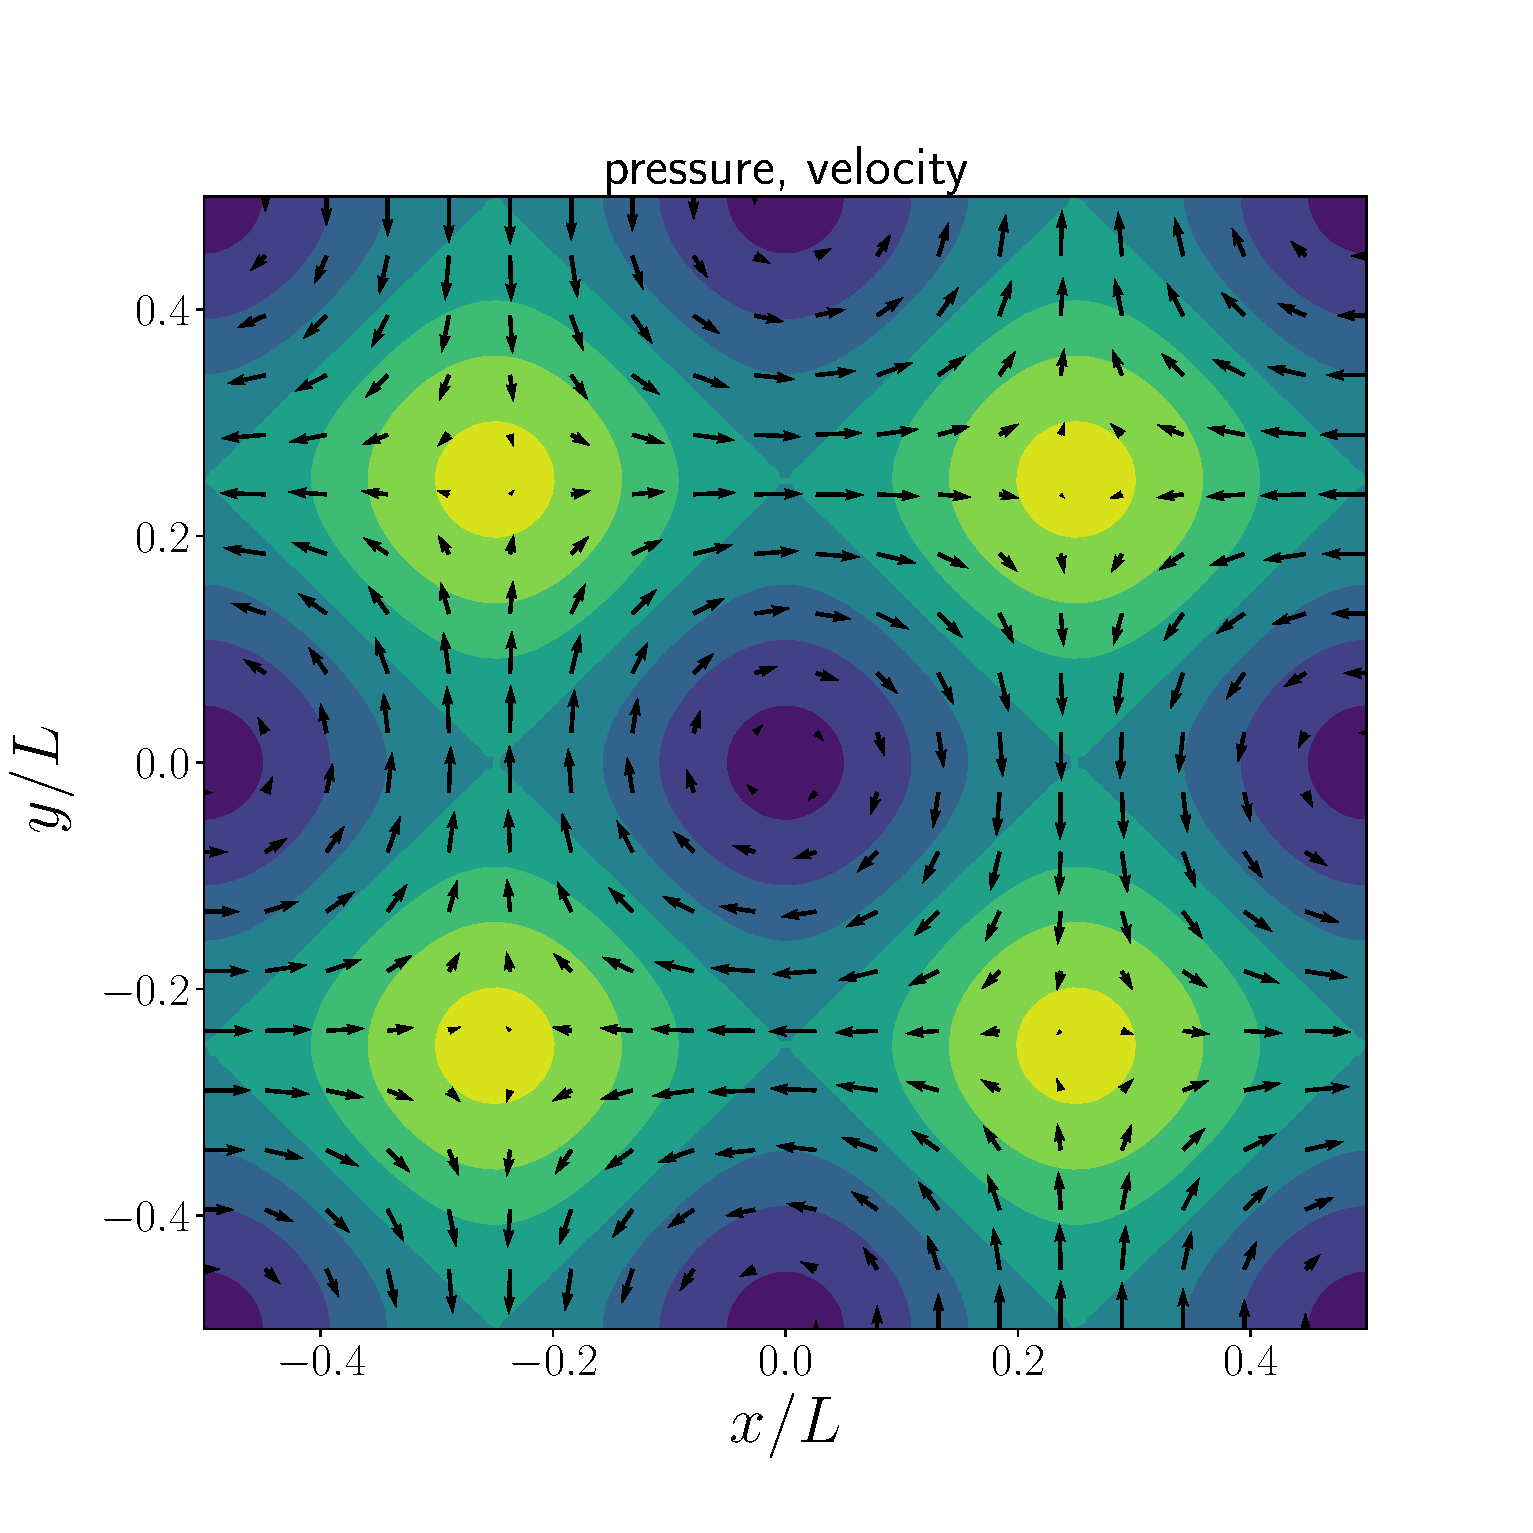
\includegraphics[width=0.4\linewidth]{figures/taylor-green_vortices}
  \caption{Taylor-Green vortices. Contour of iso-pressure (isobars),
    velocity as arrows \label{fig:taylor-green_vortices }}
\end{figure}

Insertion of these two fields into the Navier-Stokes equation shows
that indeed this is a solution. It is interesting that the pressure
gradient term exactly cancels the convective one, while the viscosity
term cancels the partial derivative. That means that in the inviscid
limit the vortices will never decay.

The vorticity field is given by
\[
  \omega = 2 f(t) \sin (kx) \sin (ky)
\]
and the stream function is just $ \psi=\omega /2$. Notice the
vorticity satisfies the convection-diffusion equation
\[
  \frac{d \omega}{d t}= \nu \nabla^2 \omega.
\]



\subsection{Reduced units}

Let us introduce the dimensionless time, built from time, maximum
initial velocity, and typical length $L$ (another choice would be
$L/2$, which is the actual length of a vortex)
\[
  t^*= t u_0 / L.
\]
Notice that $ t^*=1$ is the time a fluid particle would need to travel
a distance $L$.

Function $f$ can be written as
\[
  f(t)= \exp(-2\nu (2\pi/L)^2 (L t^* / L) ) = \exp(-8 \pi^2 t^* / \mathrm{Re}) ,
\]
%
where the Reynolds number appears naturally:
%
\[
  \mathrm{Re} := L u_0 / \nu .
\]

The decay time is then seen to be $ \tau^*=\mathrm{Re}/(8\pi^2)$ in
reduced units.




\section{Attenuation of sound waves*}
\label{sec:sound_waves_att}

This section contains a simple discussion of the role of viscosity in
the attenuation of sound waves. Original work is by Stokes, 1845.

Let us start with the Navier-Stokes momentum equation, which will be
linearized by disregarding high-order deviations from equilibrium
values. The two viscosity coefficients always multiply the velocity
terms. Therefore, they are at to be taken at their equilibrium values,
since any departure would entail higher order terms. This points out
\ref{eq:NS_const_viscs} as our starting point --- even if this case
is not athermal, the fact that the variation of the viscosity
coefficients is neglected leads to the same equation.


After linearizing, the two relevant equations are continuity and
momentum:
\begin{align}
  & \frac{\partial\rho' }{\partial t}  + \rho_0 \divu =0 \\
  & \label{eq:NS_Newtonian_const_visc}
    \rho_0 \frac{\partial \bfu }{\partial t} =
    - c^2 \nabla \rho' + \mu \nabla^2 \bfu
    + ( \mu + \lambda ) \nabla ( \divu ) .
\end{align}
The same assumptions as those in
Eqs. \ref{eq:sound_small_u}-\ref{eq:sound_small_p} have been made.
Also, we write $\kappa = c^2$ for the proportinality of pressure
modulations with density modulations, where $c$ is the sound speed
when viscosity is neglected. The subscript ``$_0$'' is not written for
the viscosity coefficients for simplicity.

Eq. \ref{eq:NS_Newtonian_const_visc} may seem different from previous
expressions, but it is the correct one when $\mu$ is constant, but
incompressibility does not hold. In this case, the term in
\ref{eq:NS_Newtonian} is not zero, but rather gives rise to a
$(\mu + \lambda) \nabla ( \divu )$ term.

Our systems is not as simple as the one in Section
\ref{sec:sound_waves}, where the continuity and momentum equations
where equally simple. There, we could easily eliminate either the
velocity or the density from our equations in order to get a single
equation for the other field. Now, the continuity equation is the
same, but the one for momentum one is much more involved. This leaves
us with eliminating the density as the only viable scheme.

If we apply the gradient operator to continuity, and differentiate
with respect to space in momentum, we arrive to this equation for
the velocity only:
\begin{equation}
  \label{eq:sound_att_Fourier}
  \frac{\partial^2 }{\partial t^2 } \mathbf{u} =
  c^2\nabla \cdot (\divu) + \nu \nabla^2\frac{\partial\bfu}{\partial t} +
  (\zeta - \nu) \nabla (\nabla\cdot \frac{\partial\bfu}{\partial t} ) ,
\end{equation}
where $\nu=\mu/\rho_0$, the usual kinematic viscosity, and we define,
for future convenience, an additional kinematic viscosity
$\zeta=2 \nu+\lambda/\rho_0$.

Clearly, this reduces to our previous sound wave equation if there was
no viscosity.

Let us try a harmonic wave solution of the form
\begin{equation}
  \label{eq:wave_form_visc}
  \bfu = \Re\left[ \bfu_0 e^{i( \beta x - \omega t)} \right].
\end{equation}
Now $\bfu_0$ is a fixed amplitude and polarization vector, which may
be parallel to $\bhe$ in a longitudinal sound wave, but may also be
perpendicular to it, for a traverse wave. In general, of course, a
wave may be a combination of both.

Notice the usage of complex exponentials, which is common in wave
physics. Of course, the actual solution is real, so usually the real
part of the complex solution is kept (sometimes it is the imaginary,
which is equally valid). The flexibility comes partly from the fact
that $\mathbf{u}_0$ could be complex, which would represent a phase.
In our case, this is not important, but rather the possibility that
$\beta$ may be complex. In this case, its values encapsulates both a
real wave number and an spatial decay. Indeed, if
\[
  \beta = k + \alpha i ,
\]
then
\[
  \bfu = \bfu_0e^{- \alpha x} e^{i(k x - \omega t )} ,
\]
which clearly identifies $ \omega=2\pi /\lambda$ as the (real)
wave-number for a wave-lenght $ \lambda$, and $ \alpha=1 /\ell $, as a
sound attenuation coefficient, with $ \ell $ the attenuation length.
\index{sound attenuation coefficient}
\index{attenuation length}

Now, the time derivative is
\[
  \frac{\partial \bfu  }{\partial t }  = -i \omega \bfu ,
\]
and the second derivative,
\[
  \frac{\partial^2 \bfu   }{\partial t^2 }  = -\omega^2 \bfu.
\]

But, it is quite interesting that the two second space derivatives are
not the same. The Laplacian is
\[
\nabla^2 \bfu = -\beta^2 \bfu,
\]
while the gradient of the divergence is
\[
\nabla (\nabla\cdot \bfu ) = -\beta^2 u_x \bhe_x,
\]
where $u_x= \bfu\cdot \bhe_x$ is the longitudinal component of the
sound wave.
%
The latter then acts only on longitudinal waves: tranverse waves are
inherently divergence-free, since depend on one coordinate but point
toward a perpendicular direction (as in Couette and Poiseuille flows).
Let us consider them separately.

\subsection{Longitudinal waves}

In this case, insertion of the wave form \ref{eq:wave_form_visc} into
Eq. \ref{eq:NS_Newtonian_const_visc} yields

\begin{equation}
  -\omega^2 = - c^2\beta^2 + i \zeta  \omega \beta^2 .
\end{equation}
The expression includes the volume bulk viscosity, as seems fitting
for a longitudinal disturbance, which involves compression.  The
appearance of the shear viscosity may come as a surprise \footnote{%
  To be precise, the fact that $\eta$, the volume viscosity, is not
  the only viscosity coefficient that appears, this beign a bit
  obscured by our usage of $\zeta$ instead of $\mu$ and $\eta$.}  The
tensor $\mu$ term in Eq. \ref{eq:pure_stress_pure_compression},
despite being traceless, nevertheless has a non-zero divergence, as
can be easily checked.  This means this wave does not consist of pure
compression, in spite of its appearance: it is also a shear wave (see
Exercises \ref{ex:shear_in_wave} and \ref{ex:div_of_traceless}.)


If viscosities were negligible, the solution is just
\[
\omega =  c \beta ,
\]
%
the usual dispersion relation for sound of
Sec. \ref{sec:sound_waves}. In general, though:
\begin{equation}
  \label{eq:waves_att_dispersion}
  \beta^2 =
  \frac{\omega^2}{c^2 - i \zeta\omega}=
  \frac{\omega^2}{c^2}\frac{1}{1 -  i\omega/\omega_\mathrm{c}},
\end{equation}
where we define the crossover angular frequency \index{crossover
  angular frequency}
\[
  \omega_\mathrm{c} := \frac{c^2}{ \zeta }.
\]

This is the frequency above which the viscosity begins to be relevant.
Numerical values can be found in Table \ref{tbl:sound_att}. The
frequency is really high for the human hearing range, which goes up to
about $\SI{20}{\kilo\hertz}$ for humans. The record in the animal
kingdom is held by porpoises (\ref{fig:porpoises}), but it is only
about $\SI{160}{\kilo\hertz}$. Ultrasonic cleaners used in dentistry
operate at $\SI{40}{\kilo\hertz}$. Medical ultrasound for imaging goes
as high as $\SI{16}{\mega\hertz}$. Only acoustic microscopy
\cite{wiki:AM} reaches a few \si{\giga\hertz}, matching our estimate
for air.


\begin{figure}
  \begin{center}
    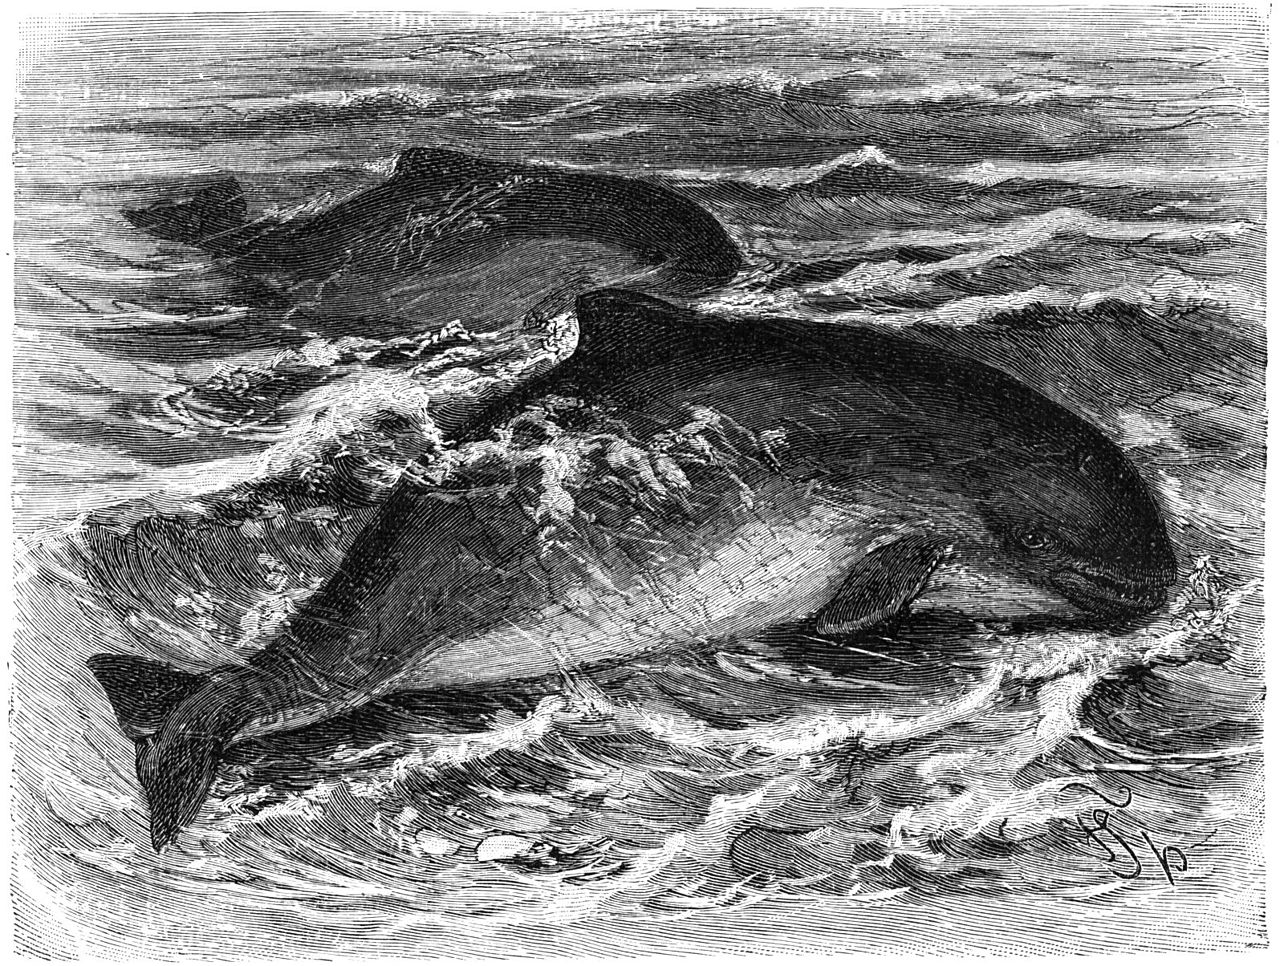
\includegraphics[width=0.7\textwidth]{figures/porpoises}
  \end{center}
  \caption{Harbor porpoises. From \cite{Brehms_Tierleben}.  \label{fig:porpoises}}
\end{figure}


\begin{table}
\begin{tabular}{|c|c|c|c|c|}
  \hline
    & $ c$ (m/s) &  $ \nu$ (m$^2$/s) & $\lambda$ (m$^2$/s) & $ f_\mathrm{c}$ (GHz)\\
  \hline
  \hline
  water (15$^\circ$C) & $1480$& $ 1.13 \times 10^{-6}$ & $ 3.1 \times 10^{-6}$ & $68$ \\
  \hline
  air & $340$   & $ 1.48\times 10^{-5}$ & $ 5 \times 10^{-6}$ ? & $0.5$ \\
  \hline
\end{tabular}
\caption{Numerical values for two important substances. Values with
  question marks are speculative, since in Cramer\cite{Cramer} air is
  said to have a negligible bulk viscosity\ldots but in a graph this
  quantity's value is seen to be about half the shear viscosity value,
  and air is mostly nitrogen.
 \label{tbl:sound_att}}
\end{table}

It is somewhat tedious to find the real and imaginary parts of $\beta$
from Eq. \ref{eq:waves_att_dispersion} (the general solution is shown
in Figure \ref{fig:sound_wave_att}.)  The resulting expressions are,
moreover, not very iluminating except at low and high frequencies
(with respect to $\omega_\mathrm{c}$). We find it better then to study
these two limits from approximations to
Eq. \ref{eq:waves_att_dispersion}, and leave the general solution as
Exercise \ref{ex:sound_att}, for the interested reader.

\begin{figure}
  \centering
  \begin{minipage}{0.7\textwidth}
      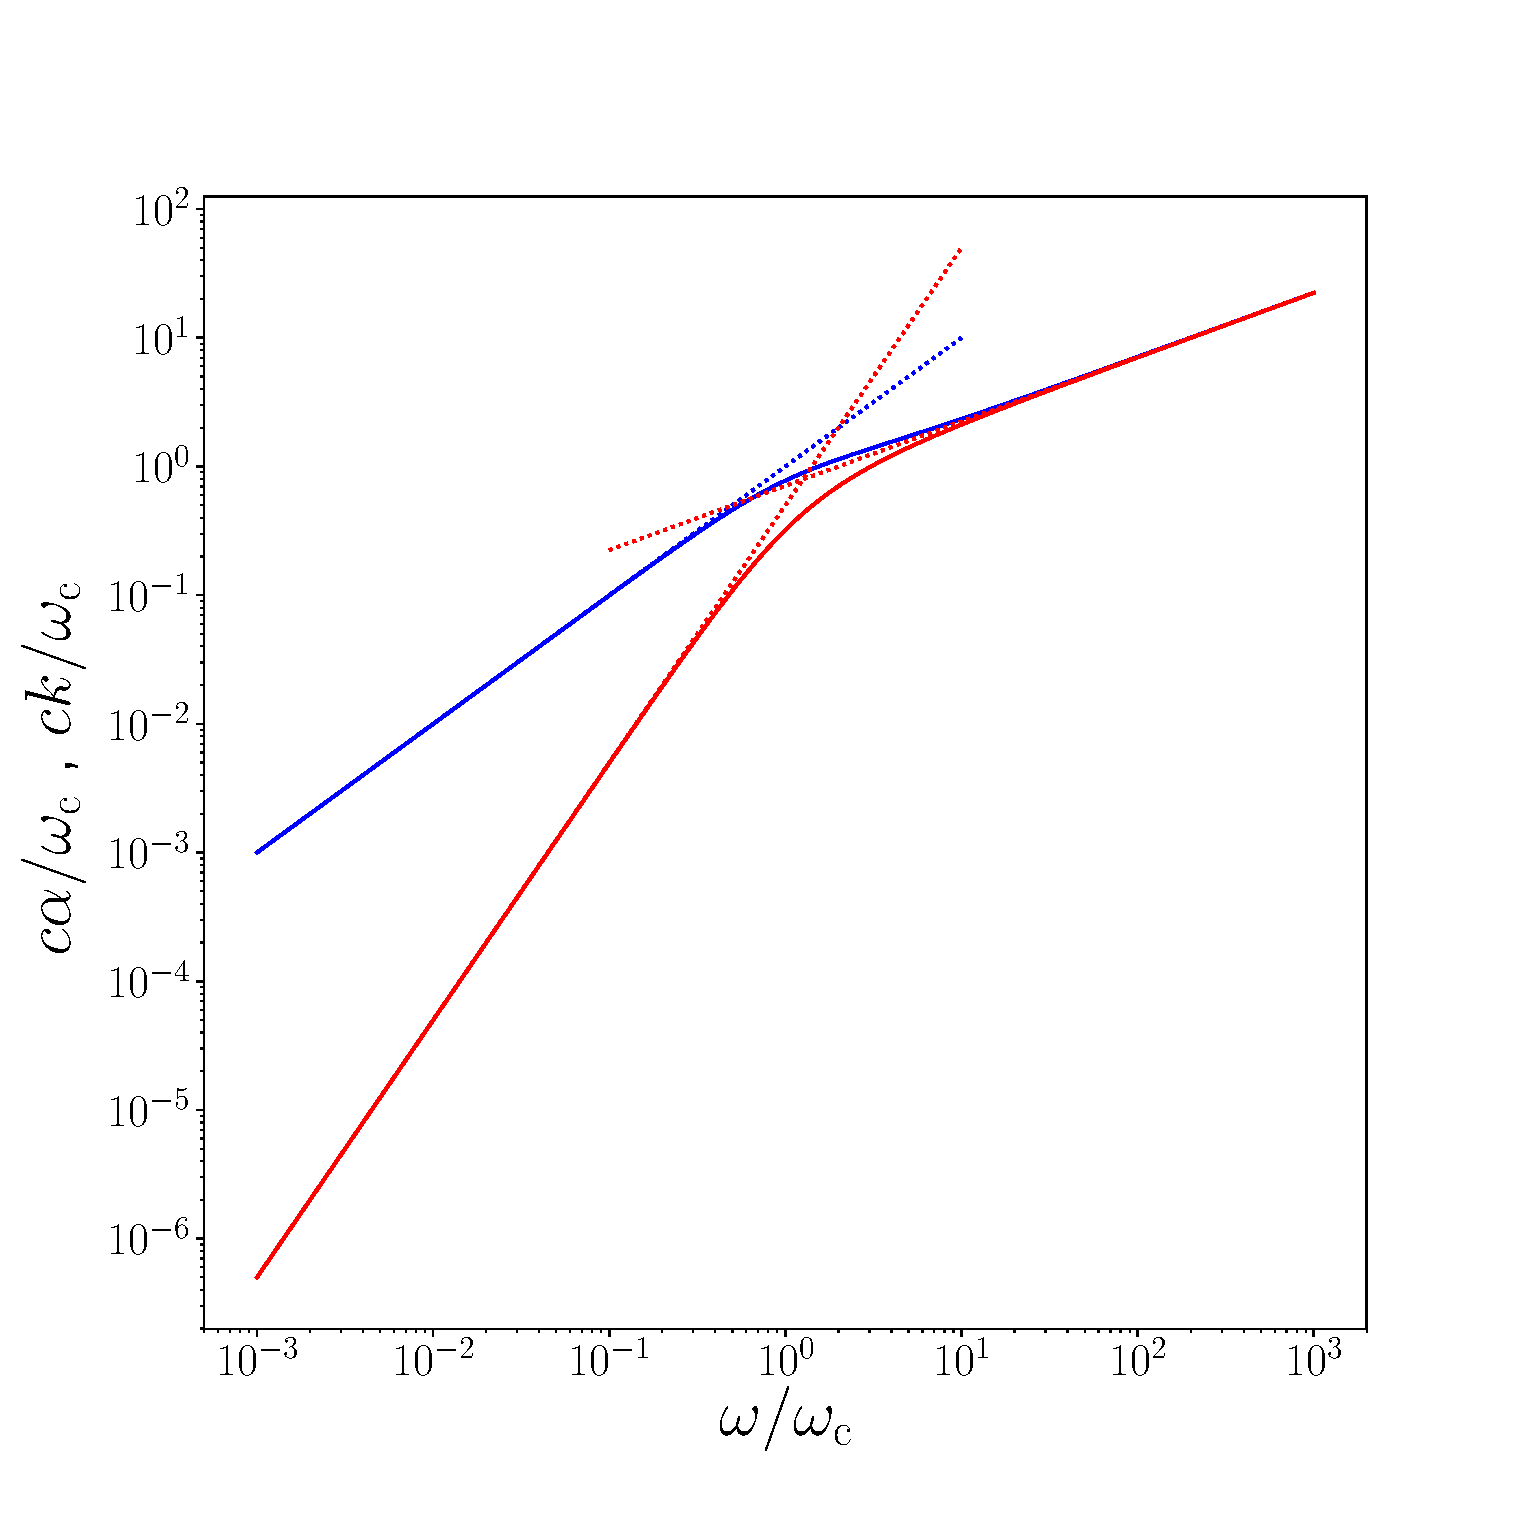
\includegraphics[width=\textwidth]{figures/sound_wave_att}
  \end{minipage}
  \caption{Plot of reduced wave-vector, $k c /\omega_\mathrm{c}$ (blue), and
    attenuation coefficient, $\alpha c /\omega_\mathrm{c}$ (red), as functions
    of reduced frecuency $\omega /\omega_\mathrm{c}$. Dotted lines are
    assymptotic regimes at low and high frequencies.
    \label{fig:sound_wave_att}}
\end{figure}


\subsubsection{Low frequencies}


At frequencies much below the crossover frequency, we may expand the
term in the denominator in a Taylor series, then again for the square
root. The end result is
\[
\beta = \frac{\omega}{c} \left(1 + i   \frac{\omega}{2 \omega_\mathrm{c}}\right).
\]
%
Therefore, the wave number is
\[
\beta = \frac{\omega}{c},
\]
as if there were no viscosity (this corresponds to the dotted blue
line at low frequencies in Figure \ref{fig:sound_wave_att}).

The attenuation coefficient is
\[ \alpha = \frac{\omega^2}{2 c\omega_\mathrm{c}}=
\frac{ \zeta \omega^2 }{2 c^3}. \]
%
It therefore grows as the square of the frequency (red dotted blue
line at low frequencies in Figure \ref{fig:sound_wave_att}).  This
agrees is called ``Stokes' law of sound'' \index{Stokes' law of
  sound}. Notice that the alternative form is often found
\cite{wiki:SLoSA}:
\[
  \alpha =  \frac{\omega^2}{\rho_0 c^3}
  \left( \frac23 \mu+ \frac12 \eta  \right),
\]
with $\eta= (2/3) \mu + \lambda$ the volume compressiblity.

This means that for that the highest sound in a porpoise's range, at
$\SI{160}{\kilo\hertz}$ the attenuation length would be about
$\SI{8}{\kilo\meter}$ (in water, of course). This may be important for
the long-range communication of these animals. For medical ultrasound
at $\SI{16}{\mega\hertz}$ this length is
$\approx\SI{80}{\centi\meter}$, with water values (a fair
approximation for the human body.) This can have an impact for human
tissues, in the sense that in a distance of some tens of centimeters
the energy of the ultrasound waves is dissipated inside the body of
the patient, and may cause unwanted heating.

\subsubsection{High frequencies}

At frequencies much higher than the crossover, we may neglect the
``1'' in the denominator of \ref{eq:waves_att_dispersion}, to obtain
\[
\beta^2 = \frac{i \omega\omega_\mathrm{c}}{c^2} .
\]
If we substitute the crossover frequency:
\[
\beta^2 = \frac{\omega}{i \zeta} =\frac{i \omega}{\zeta} 
\]
Recalling $i = e^{(pi/2)i} $, the solution is
\[
\beta =\sqrt{ \frac{\omega}{ \zeta }} e^{(\pi/4)i}.
\]

Therefore
\[
k=\alpha =\sqrt{\frac{\omega}{ 2 \zeta}}.
\]

This is an interesting result, since the attenuation coefficient is
equal to the wave number (dotted black line at high frequencies in
Figure \ref{fig:sound_wave_att}).

The attenuation length is
\[
\ell= \frac{1}{\alpha}=\sqrt{\frac{ 2 \zeta}{\omega}}
\]
The function looks therefore like a simple function
\[
g(x)= f(x/\ell) \qquad  f(x) = e^{-x}\cos(x) .
\]
In Figure \ref{fig:expcos}, it is seen to decay very fast, with just
one maximum of minimum of importance.

\begin{figure}
  \begin{center}
    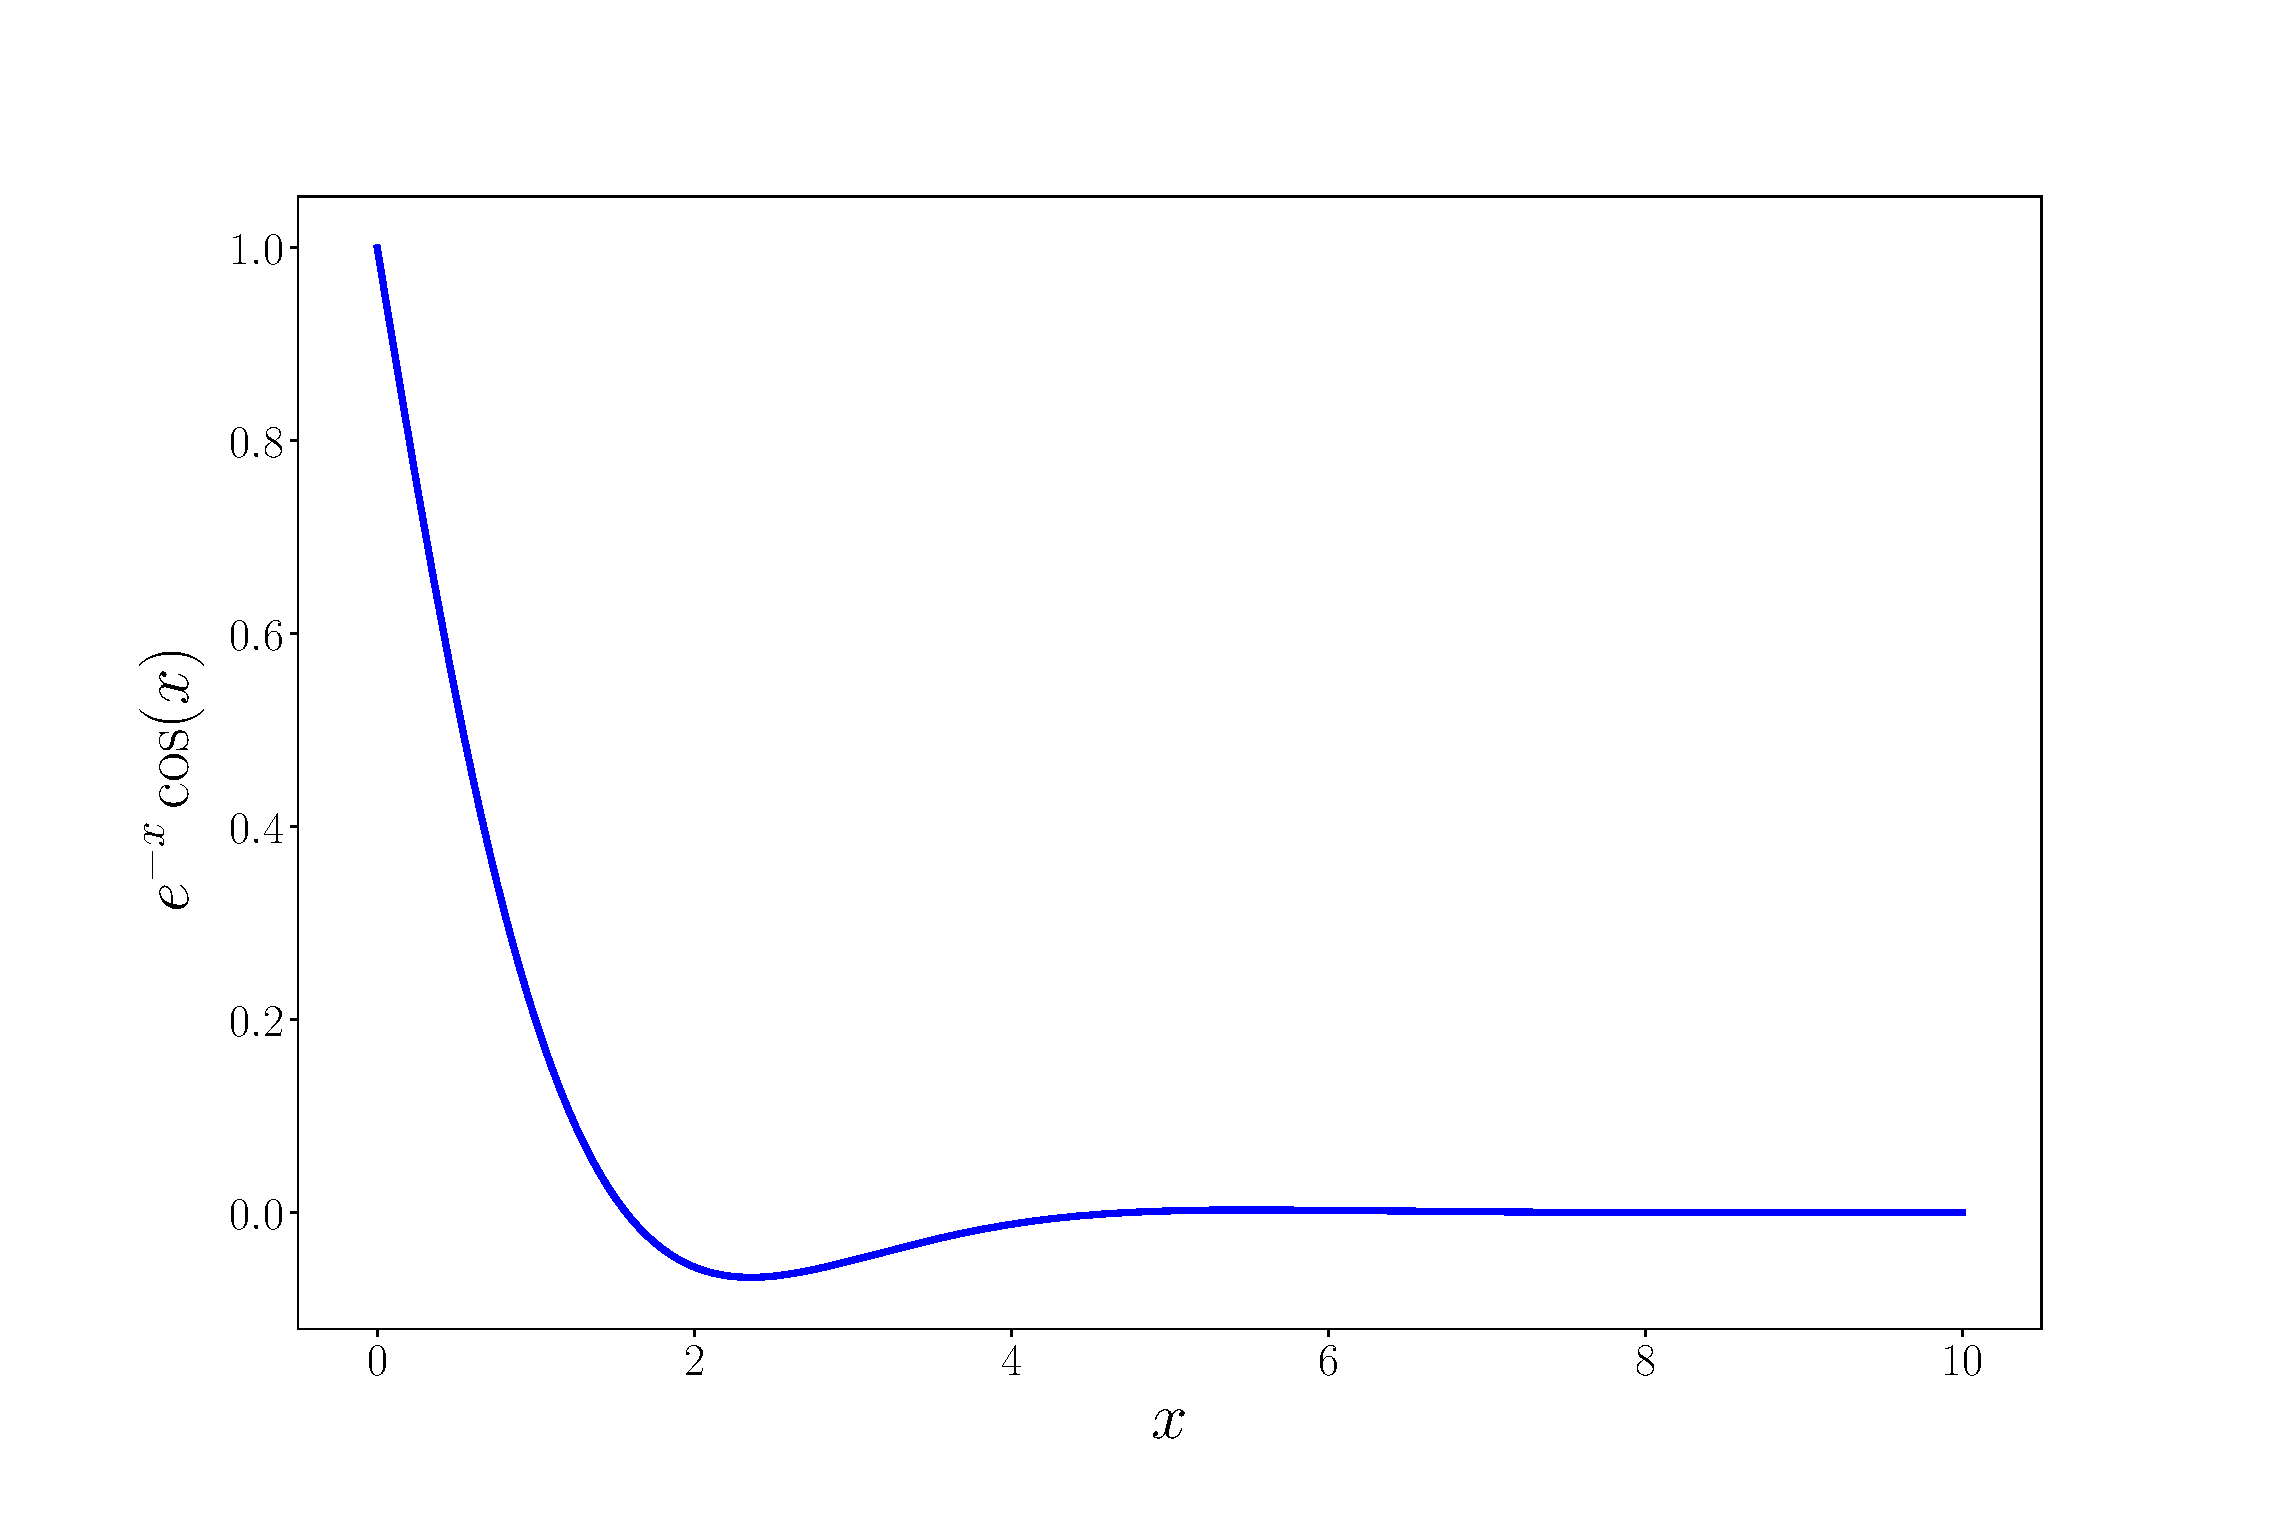
\includegraphics[width=0.7\textwidth]{figures/expcos}
  \end{center}
  \caption{Graph of the function $e^{-x}\cos(x)$ \label{fig:expcos}}
\end{figure}
 



\subsubsection{At the crossover frequency}

A fast check on the above approximations is to see what happens when
the frequency is exactly the crossover frequency. At this point, the
growth of the attenuation coefficient as the square of frequency
crosses over to a growth as the square root. This would mean a bend in
a log-log plot, between two straight lines with different slopes. This
is indeed apparent in Figure \ref{fig:sound_wave_att}.

The extrapolation of the low frequency expression yields
\[
\alpha_\mathrm{c}\approx \frac{\omega_\mathrm{c}}{2 c} ,
\]

whereas the high frequency expression yields
\[
\alpha_\mathrm{c}\approx \frac{\omega_\mathrm{c}}{\sqrt{2} c} ,
\]
which are similar.

The exact expression can be shown to be, after some involved algebra,
\[
\alpha_\mathrm{c} =\frac{ \sin(\pi/8) \omega_\mathrm{c} }{ (2^{1/4} c } ,
\]
a value just a bit below the other two. This means the approximations
remain quite fair up to the limit of their respective ranges.

By the way, for water this value corresponds to an attenuation length
of about \SI{10}{\nano\meter}, which is a really short length, in the
atomic range. For air, it is about \SI{0.3}{\micro\meter}, the size of
a very small cell.

\subsection{Transverse waves}

We tend to think sound waves are longitudinal. We here discuss how
they may have a transverse component, but it is dampened at al
frequencies.

If we write Eq. \ref{eq:sound_att_Fourier} for the $y$ or $z$
Cartesian component, we find
\[
-\omega^2 =  i \nu \omega \beta^2 ,
\]
or
\[
\beta^2 = \frac{i \omega}{\nu}.
\]
Only $\nu$ is involved, which is sensible: transverse waves do involve
only shear, not compression (at variance with longitudinal waves,
which involve both.)

The expression is very similar to the one for longitudinal waves at
high frequencies, only this one is valid at \emph{all} frequencies.
Its solution is
\[
k = \alpha = \sqrt{ \frac{\omega}{ 2 \nu}}.
\]
Figure \ref{fig:expcos} still applies to these waves, with the
difference that the decay length is
\[
\ell= \frac{1}{\alpha}=\sqrt{\frac{ 2 \nu}{\omega}}
\]

For frequencies of ordinary ``sound'', i.e. audible frequencies, that
length is quite small. With the numerical data in the Table, that
length is only about \SI{0.7}{\milli\meter} for air, at a very low
frequency of \SI{10}{\hertz} (just below the lower hearing threshold),
and will decrease further as the inverse of the square root of the
frequency.




\section{Exercises}

\begin{enumerate}

	\item Prove the expression for the unsteady Couette flow.
	
	\item \label{ex:shear_in_wave} Write down the pure-shear stress tensor
	(see also Eq. \ref{eq:pure_stress_pure_compression}):
	\[
	\tau_\mathrm{ps} :=
	\mu  \left[
	\left(
	\nabla\bfu + \nabla\bfu\tran  - \frac23 (\divu)  \eye
	\right)
	\right] 
	\]
	for our linear wave \ref{eq:wave_form_visc} in the case it is
	longitudinal. Show that it is traceless (which it must, by
	definition), but non-zero. This latter fact indicates that our wave
	is not purely compressive in nature.
	
	\item \label{ex:div_of_traceless} Show that the volumetric force due
	to the previous pure-stress is
	\[
	\mu \nabla \cdot  \tau_\mathrm{ps}  = -\frac43 \mu \beta^2 \bfu
	\]
	
	\item \label{ex:sound_att} Find the general solution of
	Eq. \ref{eq:waves_att_dispersion} for the real and imaginary parts
	of $\beta$. Hint: use reduced quantities $\beta'= c\beta/\omega $,
	$\omega'=\omega/\omega_\mathrm{c}$, in terms of which the equation
	reads simpler:
	\[
	\beta'^2 = \frac{1}{1-i \omega'} .
	\]
	Then, write $\beta'=k'+i \alpha'$, find its square, and equate real
	and complex parts on both sides of the equation.  The solution is
	\begin{align*}
		2\alpha'^2 &=\frac {1}{\sqrt{1+\omega'^{2}}} - \frac {1}{1+\omega'^{2}} \\
		2k'^2     &=\frac {1}{\sqrt{1+\omega'^{2}}} + \frac {1}{1+\omega'^{2}}
	\end{align*}
	
	
\end{enumerate}

\chapter{The overdamped limit}

The low Reynolds number is called the creeping, or over-damped
regime. Let us generalize slightly the momentum equation
Eq \ref{eq:NS_usual} to a general volumetric external force $\bff$:
\[
  \rho \frac{d\bfu }{dt} =
  - \nabla p 
  + \mu \nabla^2 \bfu
  + \bff .
\]

We may again cast the equation into reduced form, to get
\[
\rho^* \frac{d\bfu^* }{dt^* } =
-  \nabla^* p^*
+  \frac1\mathbf{Re} \nabla^{*2} \bfu^* .
+  \bff^* ,
\]
where $\bff^*= L/(\rho_0 u_0^2) \bff$. 

As $\mathbf{Re}$ is very small, the equation will tend to
\[
0 = - \mathbf{Re} \nabla^* p^* + \nabla^2 \bfu^* + \mathbf{Re} \bff^*
.
\]
All time derivatives are gone from the equation! The only time
variation that is sometimes considered is the case in which $\bff^*$
is a explicit function of time. In this case, the velocity field
addapts



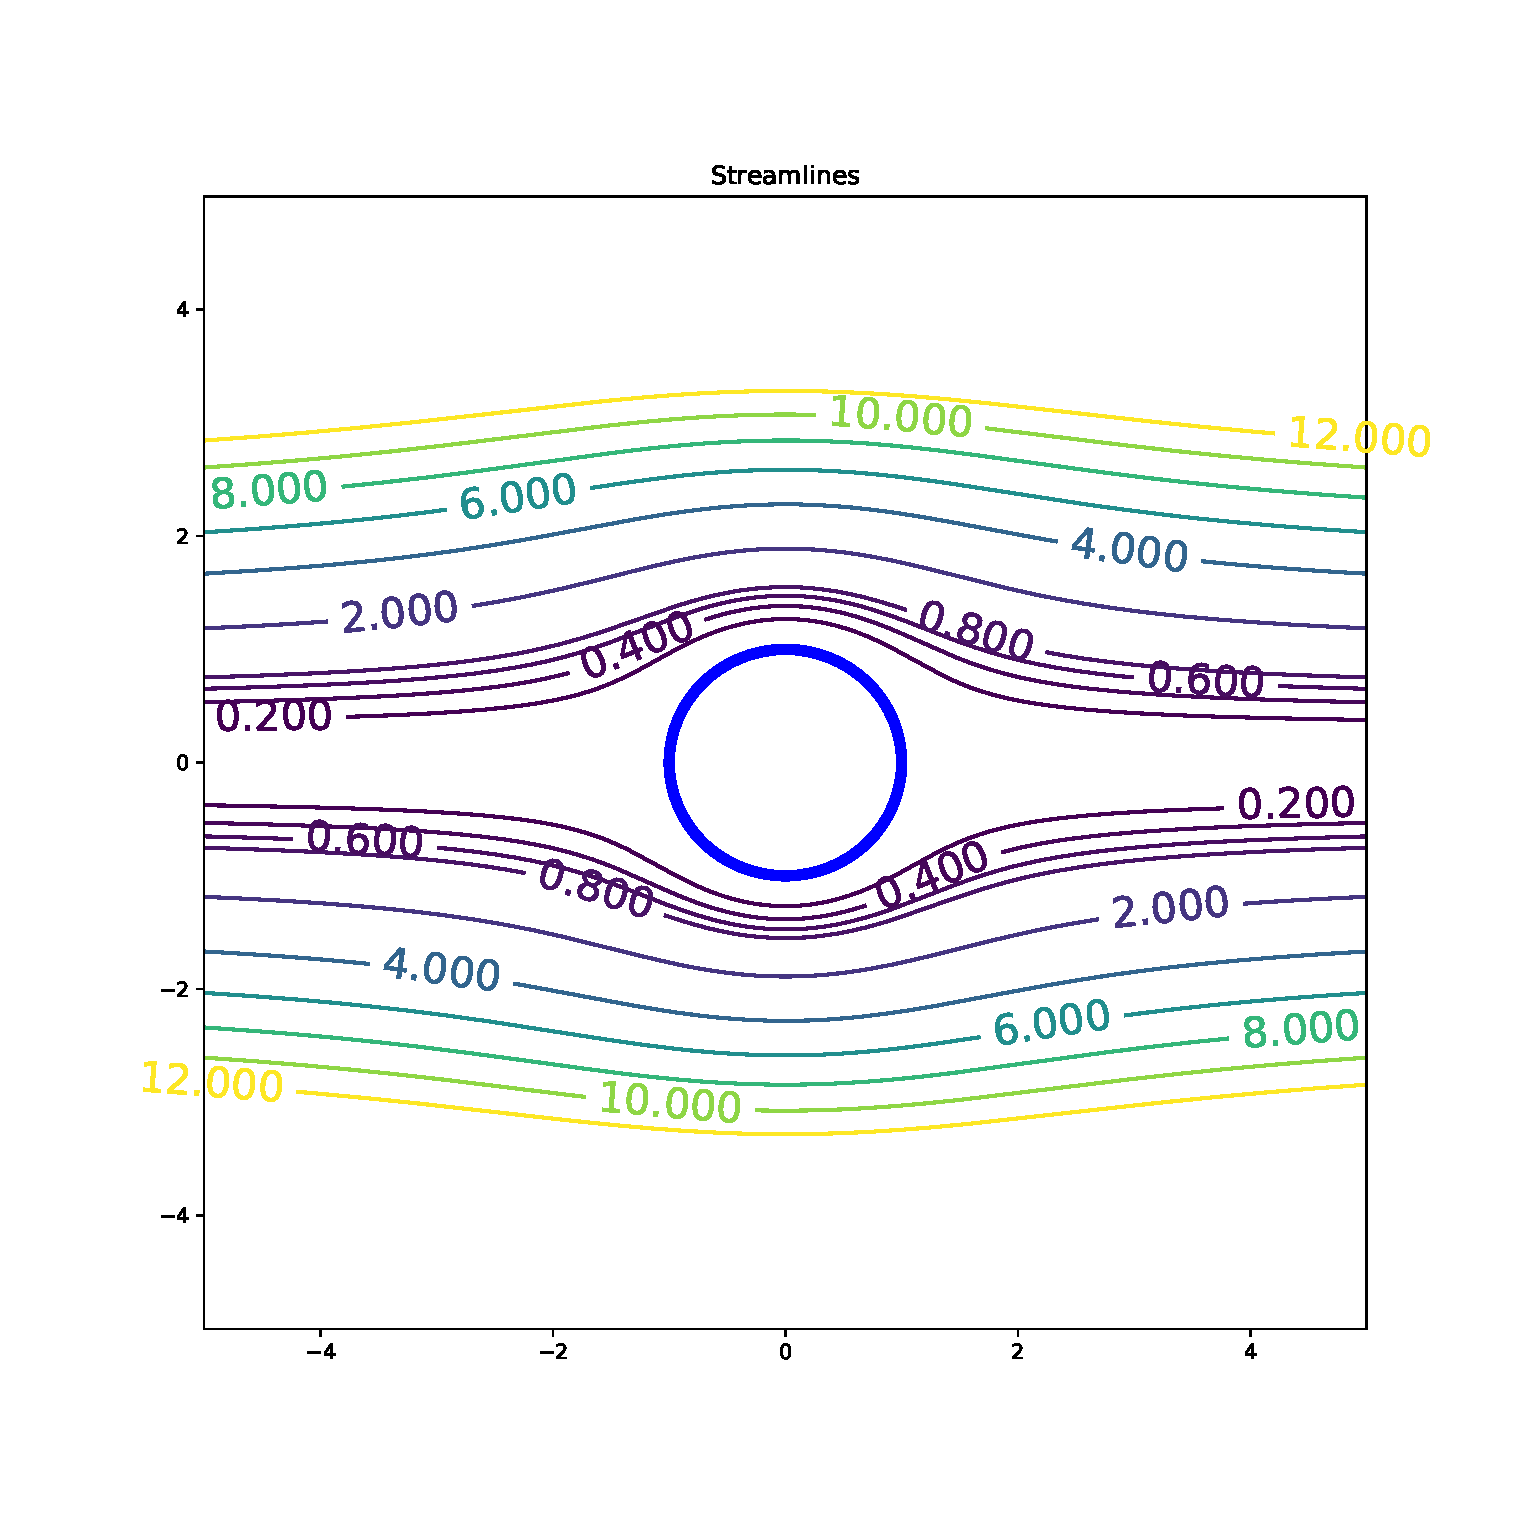
\includegraphics[width=0.8\linewidth]{figures/creeping_flow_past_sphere}

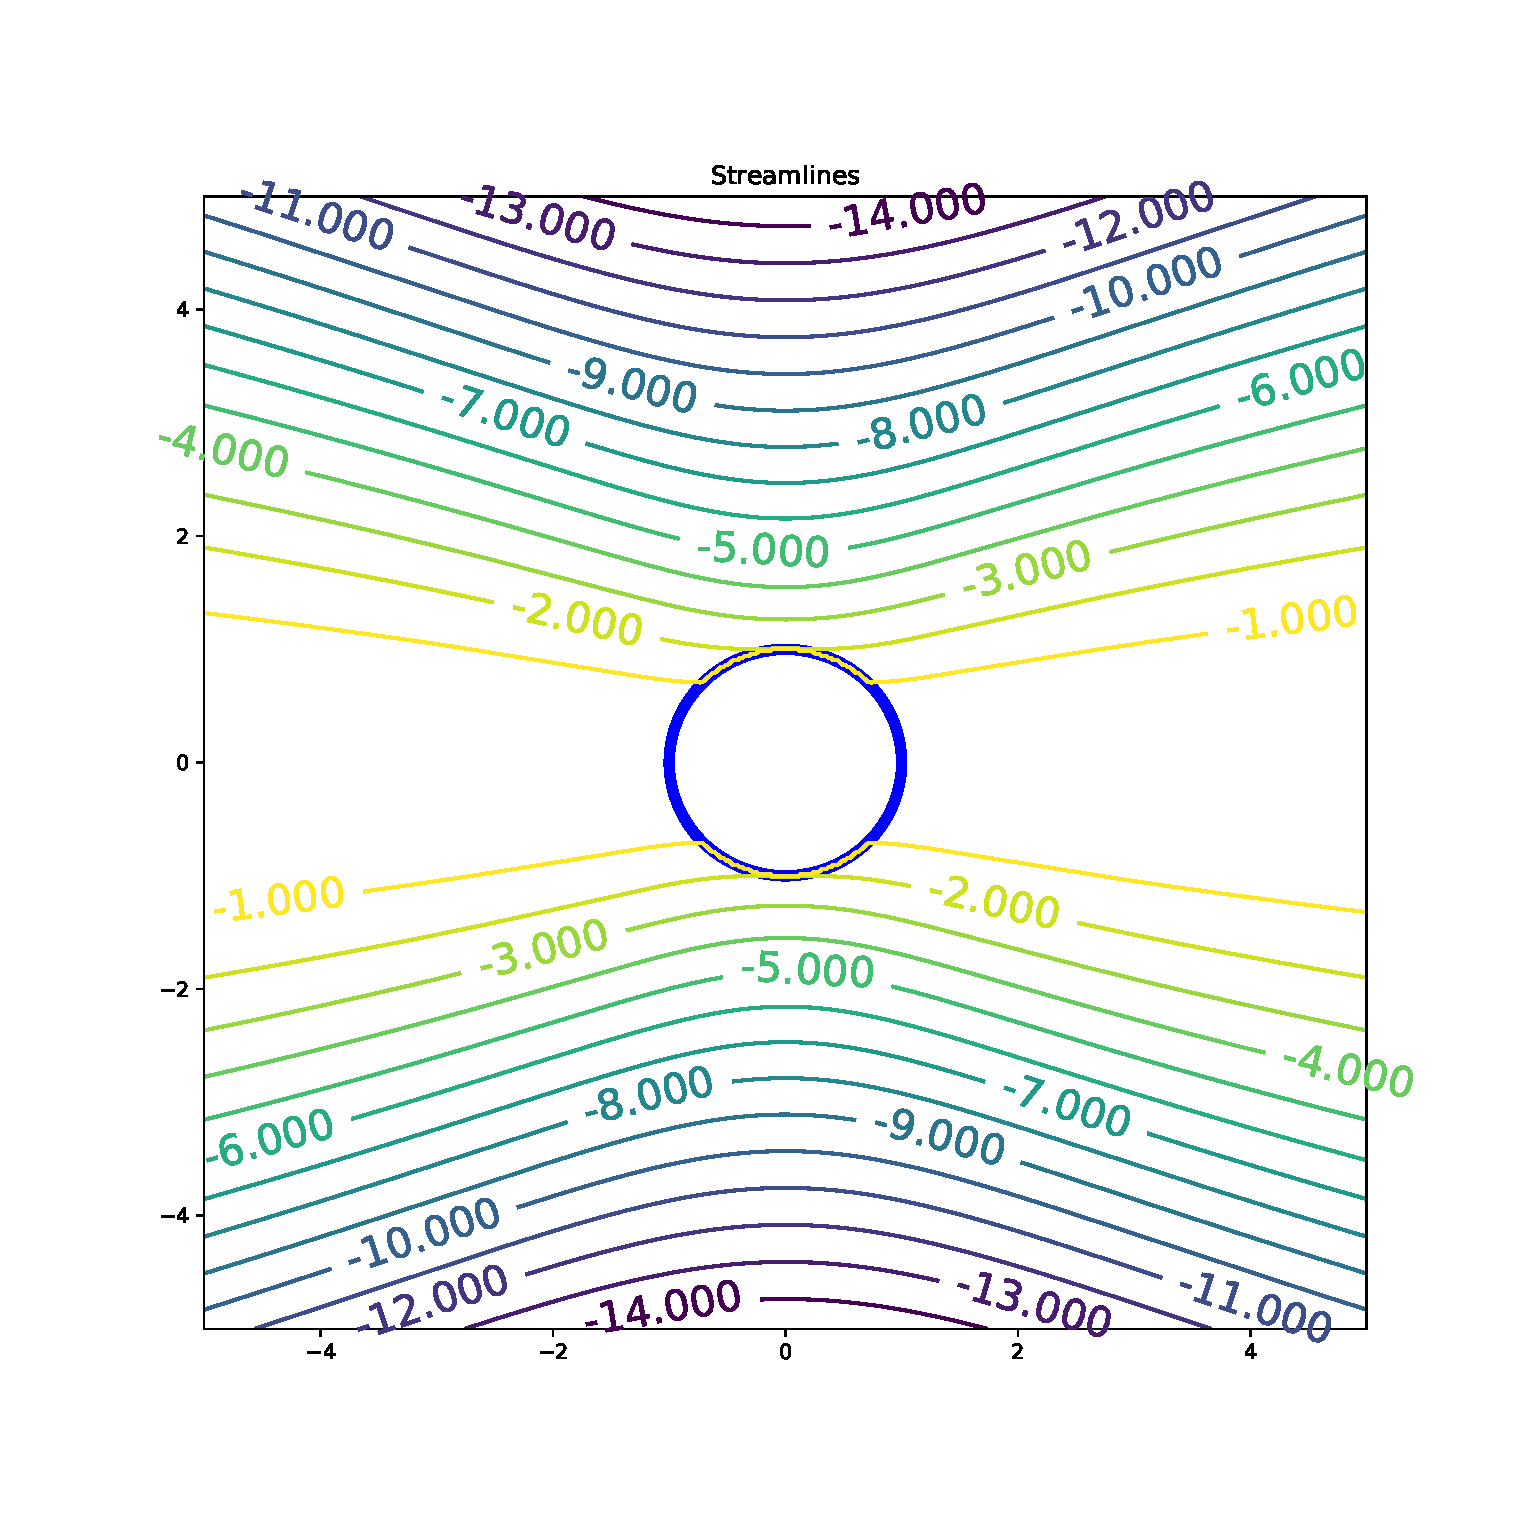
\includegraphics[width=0.8\linewidth]{figures/creeping_flow_past_sphere_moving}







\subsection{Kolmogorov flow}

In order to get an idea of the features of the flow (typical speed,
time scale, Reynolds number), we may gain some insight from the
solution from Kolmogorov flow.

This is an exact solution of the momentum equations when there is a
periodic applied force in the $x$ direction that depends on $y$ only
\[
\bff = f_0 \cos(2\pi y/L) \mathbf{e}_x .
\]

In this case, the typical lengthscale $L_0$ and velocity $u_0$ are set
by the force. The former is clearly $L_0=L$, but the velocity is
actually part of the solution. It is therefore more convenient to
introduce an alternative way to cast the momentum equation in
non-dimensional form. First, dividing by $f_0$ and going to
dimensionless spacial coordinates:
\begin{equation}
\label{eq:Navier-Stokes_nondim1}
\frac{\rho}{f_0}
\frac{d \bfu}{d t} =
\frac\eta{f_0 L^2} (\nabla^*)^2 \bfu
-\frac 1{f_0 L} \nabla^* p + \bff^*(\bfr^*) .
\end{equation}
The viscous term sets the velocity scale: $u_0 = ( f_0 L^2 ) / \eta $.
On the left hand side the total derivative limits the setting of the
time scale. Indeed, $t_0=L/u_0$, or else the two terms in the
derivative, Eq. \ref{eq:total_deriv}, have different scaling. (This
may be alright in theory, and in an Eulerian simulation, but in a
Lagrangian simulation it is not, since the advection term does not
appear explicitely.) This means the equation may be written as
\[
\frac{\rho L^3 f_0}{\eta^2}
\frac{d \bfu^*}{d t^*} =
(\nabla^*)^2 \bfu^*
-\nabla^* p^* + \bff^*(\bfr^*) ,
\]
or
\begin{equation}
\label{eq:Navier-Stokes_nondim2}
\mathrm{Re}
\frac{d \bfu^*}{d t^*} =
(\nabla^*)^2 \bfu^*
-\nabla^* p^* + \bff^*(\bfr^*) ,
\end{equation}
where we again find the Reynolds number, given as $\rho L^3 f_0 /
\eta^2$.  Notice that the reduced response time is given by the
Reynolds number: a high Reynolds number means a long reduced time to
respond, while a low Reynolds one the response is very rapid, and the
equilibrium solution is reached very fast.

To summarize, the various scales are given by:
\begin{itemize}
\item force $f_0$
\item space $L$ (therefore, the reduced del operator $\nabla^* :=
  L \nabla$),
\item velocity $u_0 = ( f_0 L^2 ) / \eta $,
\item time $t_0 = L / u_0 = \eta / (f_0 L) $,
\item pressure $p_0= f_0 L $,
\item the Reynolds number is Re=$\rho L^3 f_0 / \eta^2$
\end{itemize}


Let us apply this scaling to the Kolmogorov flow. The starting
equation for the $x$ component of the velocity, called customarily
``$u$'' is:
\begin{equation}
\label{eq:Kolmo_orig}
  \rho \frac{\partial u}{\partial t} =
  \eta \nabla^2 u - \nabla p +   f_0 \cos(2\pi y/L)  .
\end{equation}

We have supposed that the resulting velocity, as the driving force,
only has an $x$ component varying on $y$, so that the convective term
is zero. In this case, the flow is always incompressible
($\nabla\cdot\bfu =0$), so we may set the pressure to some constant
values, which thus disappears from the equation, which is just:
\[
  \rho \frac{\partial u}{\partial t} =
  \eta \nabla^2 u +   f_0 \cos(2\pi y/L)  .
\]

In reduced units (dropping the asterisks for clarity), this is
\[
  \mathrm{Re} \frac{\partial u}{\partial t} = \nabla^2 u + \cos(2\pi y) .
\]

The solution is easily found:
\[
u = \frac{1}{(2\pi)^2} \left( 1-e^{ - (2\pi)^2 t/Re } \right)  \cos(2\pi y) .
\]

Putting the scales back in, we find
\[
u = \frac{ f_0 L^2 }{(2\pi)^2 \eta}
\left( 1-e^{- (2\pi)^2 \eta  t / (\rho L^2) } \right)  \cos(2\pi y/L) ,
\]
which indeed is the solution to the original Equation
\ref{eq:Kolmo_orig}.



\chapter{The viscous boundary layer}

\section{Stagnation flow}

In order to provide a glimse into the difficulties that are
encountered as soon as one ventures into slightly more complicated
problems, let us work out a solution of Navier-Stokes equations for a
simple stagnation situation.

The potential flow solution for a stady-state incompressible 2D
stagnation flow pattern close to a flat wall is given by the stream
function
\[
\psi = B x y ,
\]
from which,
\[
\begin{cases}
  & u_x =  \frac{\partial \psi}{\partial y} =   B x \\
  & u_y = -\frac{\partial \psi}{\partial x} = - B y .
\end{cases}
\]

The parameter $B$ has units of inverse time, and is given in practical
situations by $u_0 / L$, where $u_0$ is a relevant upstream velocity,
and $L$ a relevant size.

Recalling what we learned about potential flow and its relationship
with complex analysis, since $\psi = (B/2) \Im (z^2)$, it is easy to guess the
correct potential: $\phi=\Re( z^2) = (B/2) (x^2 + y^2)$.

This flow pattern looks roughly correct, see
Fig. \ref{fig:stagnation_streamlines} left, where the streamlines are
shown, along with the pressure. The latter follows from Bernoulli
principle:
\begin{equation}
  \label{eq:p_stag_pot}
p =
 -\frac{1}{2} \left[
  u_x ^2 +
  u_y^2
  \right] =
-\frac{1}{2} \left[
  (B x)^2 +
  (-B y)^2
  \right].  
\end{equation}


\begin{figure}
  \centering
  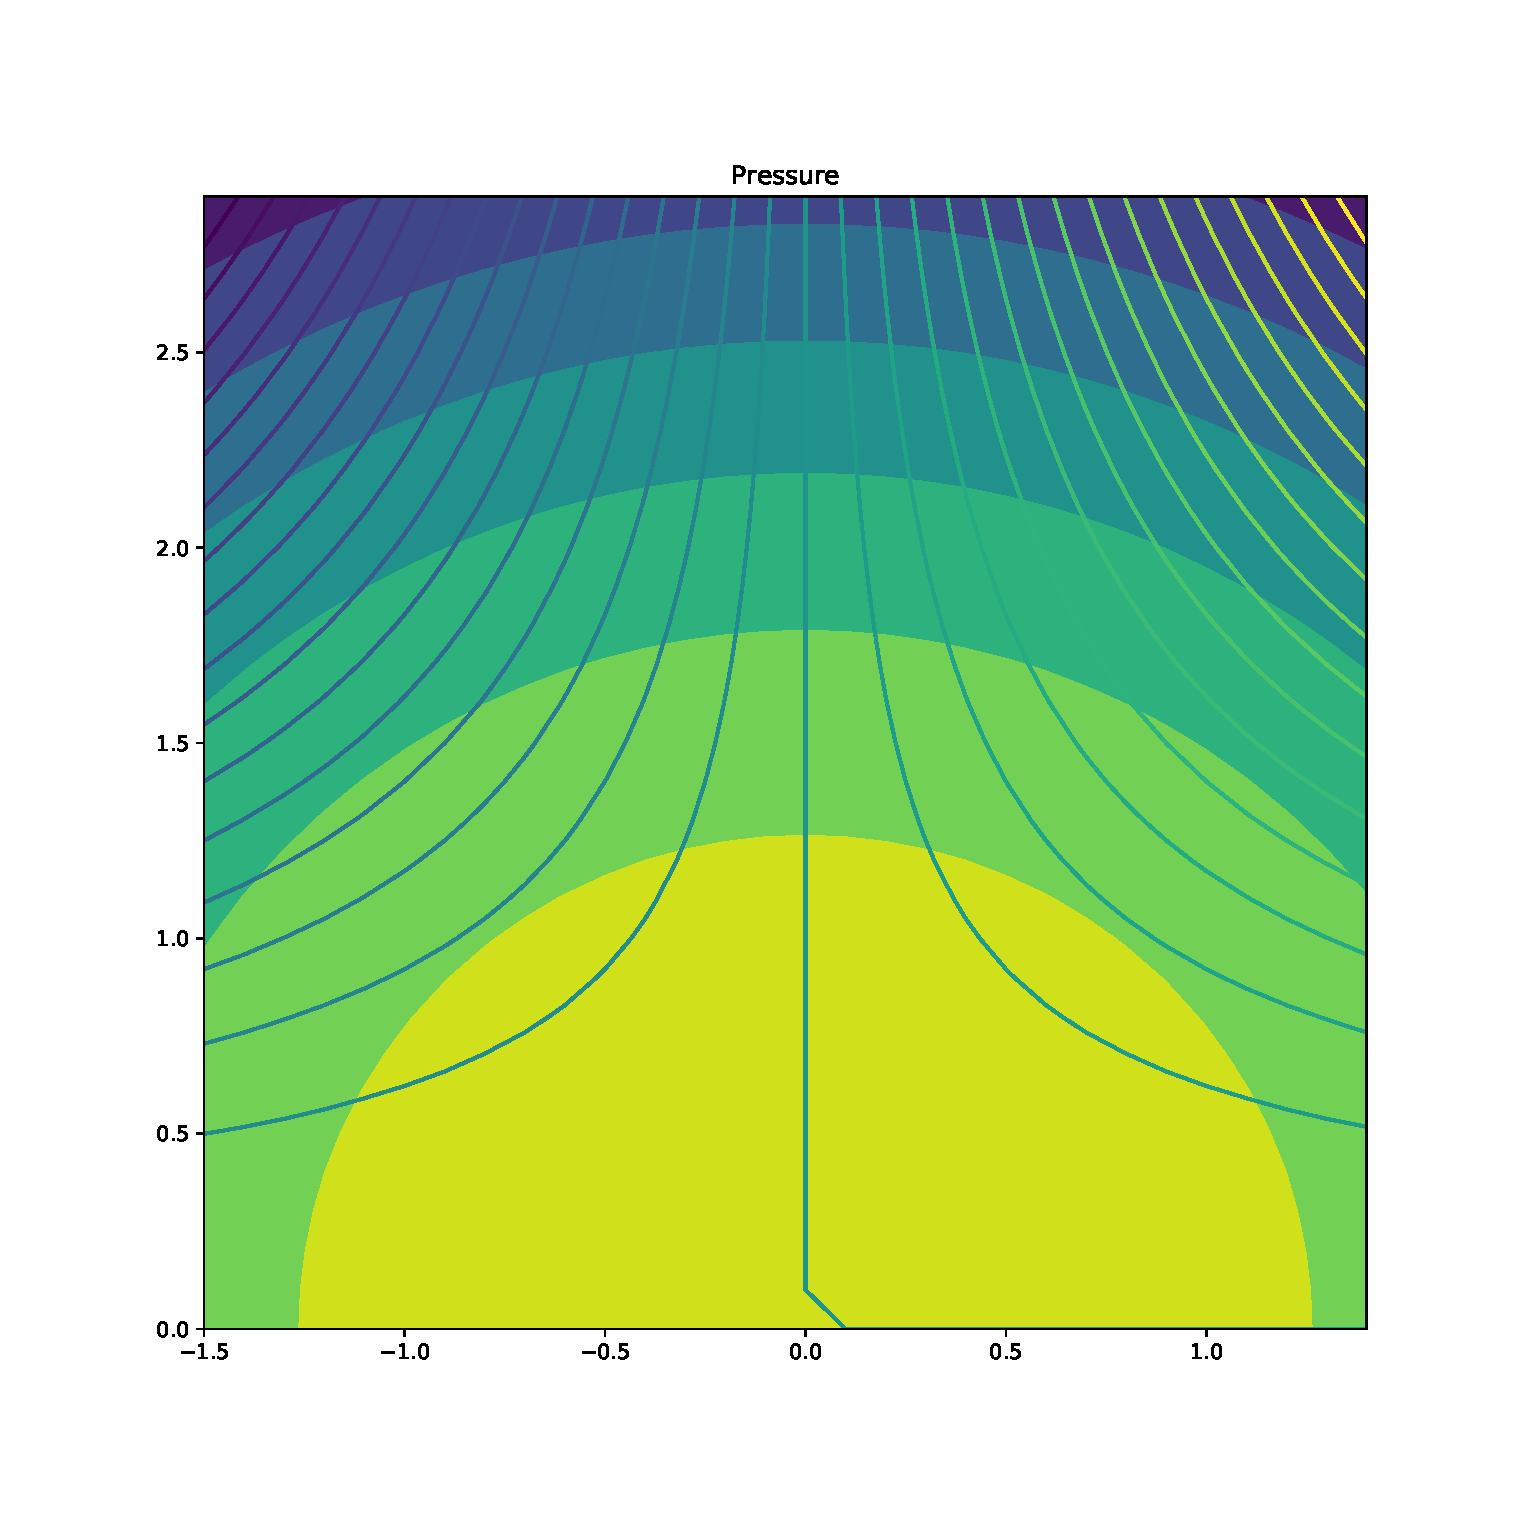
\includegraphics[width=0.4\linewidth]{figures/stagnation_potential_streamlines}
  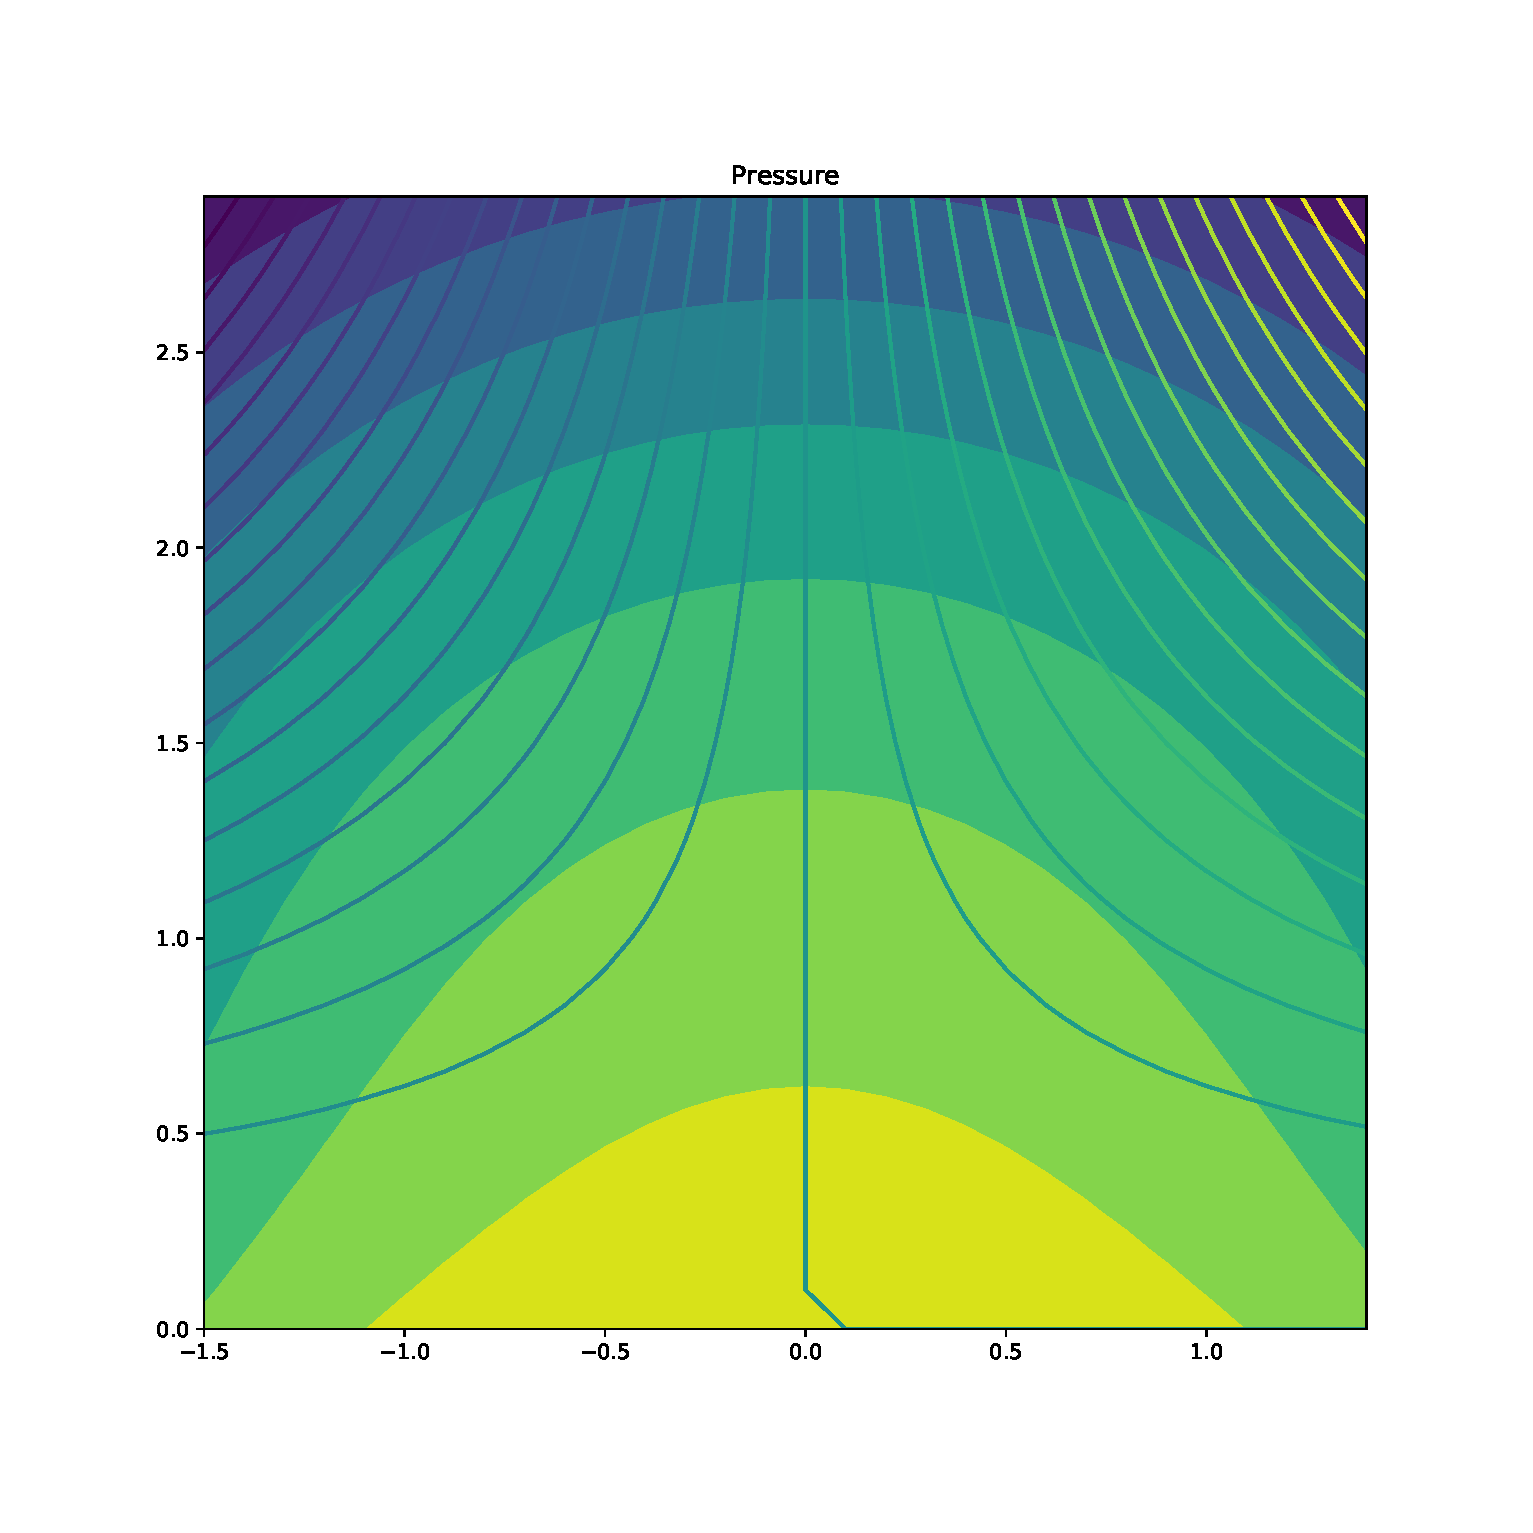
\includegraphics[width=0.4\linewidth]{figures/stagnation_viscous_streamlines}
  \caption{\label{fig:stagnation_streamlines}}
\end{figure}

But of course, at the wall ($y=0$) the fluid flows freely along the
wall. This means the boundary conditions are of the ``slip'' kind,
instead of the more realistic ``no-slip'' kind.

In order to find a correct flow, let us us the ansatz, originally
investigated by Hiemenz in 1911\footnote{%
  Hiemenz was a student of Prandtl, the founder of the theory of
  viscous boundary layers.
}.
  \[
\psi = B x f(y) ,
\]
where $f$ is a function of $y$ only. This is basically a separation of
variables, also guessing a linear dependence on $x$.

The velocity is now,
\[
\begin{cases}
  & u_x =   B x f' \\
  & u_y = - B f .
\end{cases}
\]
The correct no-slip condition then implies $f(0)=f'(0)=0$. We will
also require $f'(\infty)\to 1$ in order to recover our previous,
potential flow, solution.

Now, the steady 2D Navier-Stokes equations read
\begin{align}
  u_x  \frac{\partial u_x}{\partial x} +
  u_y  \frac{\partial u_x}{\partial y} 
  & =   - \frac{\partial p}{\partial x} +
  \nu
  \left(
  \frac{\partial^2 u_x}{\partial x^2} +
  \frac{\partial^2 u_x}{\partial y^2}
  \right) \\
  u_x  \frac{\partial u_y}{\partial x} +
  u_y  \frac{\partial u_y}{\partial y} 
  & =   - \frac{\partial p}{\partial y} +
  \nu
  \left(
  \frac{\partial^2 u_y}{\partial x^2} +
  \frac{\partial^2 u_y}{\partial y^2}
  \right) .
\end{align}
(Here, $p$ is not the true pressure, but the ``kinematic pressure'',
$p/\rho$. For convenience, a $\rho$ factor is assimilated into it, in
the same way that $\nu=\mu/\rho$.)

The $x$ equation is then reduced to
\[
 (B x f') (B f') + (-B f) B x f'' =  - \frac{\partial p}{\partial x} +
\nu B x f''' ,
\]
which may be written as
\[
B f f'' - B (f')^2 + \nu f''' = \frac{1}{B x} \frac{\partial
  p}{\partial x}  .
\]
Now, the left part of the equation is a function of $y$ only. This
means the pressure can only have this form:
\[
p(x,y) = C x^2 + h(y) ,
\]
with a constant $C$ and a function of $h$ to be determined later. Moreover,
as $y$ gets large we want to recover the potential solution. In this limit,
\[
f \to a + y \qquad f' \to 1 \qquad f'' \to 0 \qquad f'''\to 0 ,
\]
so the equation in this limit is
\[
- B \to  \frac{2 C x }{B x} ,
\]
which means $C =-B/2$, to be used later when solving for the pressure.

We must then solve
\[
 B \left(  f f'' + 1-  (f')^2 \right) + \nu f''' = 0 .
\]

Now, a lot may be learned from the shape of an equation without even
solving it. Let us look for a similarity transformation of the
form
\[
f(y) = b g(a y) ,
\]
so that equation for $f$ may be cast as an equation for $g$ with no
parameters. With this prescription,
\[
f' = ba g' \qquad f''=b a^2 g'' \qquad f'''= b a^3 g''' ,
\]
So then the equation reads
\[
 B \left(  b^2 a^2 g g'' + 1-  b^2 a^2 (g')^2 \right) + \nu b a^3  g''' = 0 .
\]
Because of the ``$1$'' in the parenthesis, it is clear $b=1/a$, so then,
\[
 B \left(  g g'' + 1-  (g')^2 \right) + \nu  a^2  g''' = 0 .
\]
Therefore, if $a=\sqrt{B/\nu}$,
\begin{equation}
  \label{eq:Z_ode}
  g g'' + 1-  (g')^2  +  g''' = 0 ,
\end{equation}
with no parameters, as we wanted. This means that, whichever solution
we find, our $f$ is going to be given by
\[
f(y) = \sqrt{\frac{\nu}{B}} g\left(\sqrt{\frac{B}{\nu}}  y  \right) =
\sqrt{\frac{\nu}{B}} g\left(\frac{y}{ \sqrt{\nu/B} } \right) =
 \ell g\left(\frac{y}{ \ell } \right) .
\]
Clearly, $\ell = \sqrt{\nu/B} $ sets the scale of variation of the
flow away from its potential solution.

Notice that the velocities will be
\[
\begin{cases}
  & u_x =   B x g'(y/\ell) = B\ell \frac{x}{\ell} g'(y/\ell)  \\
  & u_y = - B \ell g(y/\ell)  ,
\end{cases}
\]
so that the velocity scale is set by $B\ell=\sqrt{B\nu}$.


%The $y$ equation reduces, with our velocities, to
%\[
%B^2 f f' = - \frac{\partial p}{\partial y} - B\nu f'' .
%\]
%This means that $\frac{\partial p}{\partial y}$ is a function of $y$
%only.



Our task is then to integrate the non-linear ODE \ref{eq:Z_ode}, subject
to these boundary conditions:
\[
g(0)=0 \qquad g'(0)=0 \qquad g''(x\to \infty) \to 0 .
\]
If we had a condition on $g''(0)$, the problem would be a
straight-forward exercise in integration. However, we have instead a
condition on the other side of the integration domain, which makes
this problem somewhat harder. The technique should then be a
``shooting method'', in which $g''(0)$ is adjusted until a vanishing
small of $g''$ far away is found. The procedure may be made
systematic, but we can also fiddle a bit with the parameters in order
to find a reasoable approach. It is quite easy to arrive at
$g''(0)\approx 1.234$, as in the jupyter python notebook at
Supplementary Material.

%How far is far away may be again estimated from the equation.


\begin{figure}
  \centering
  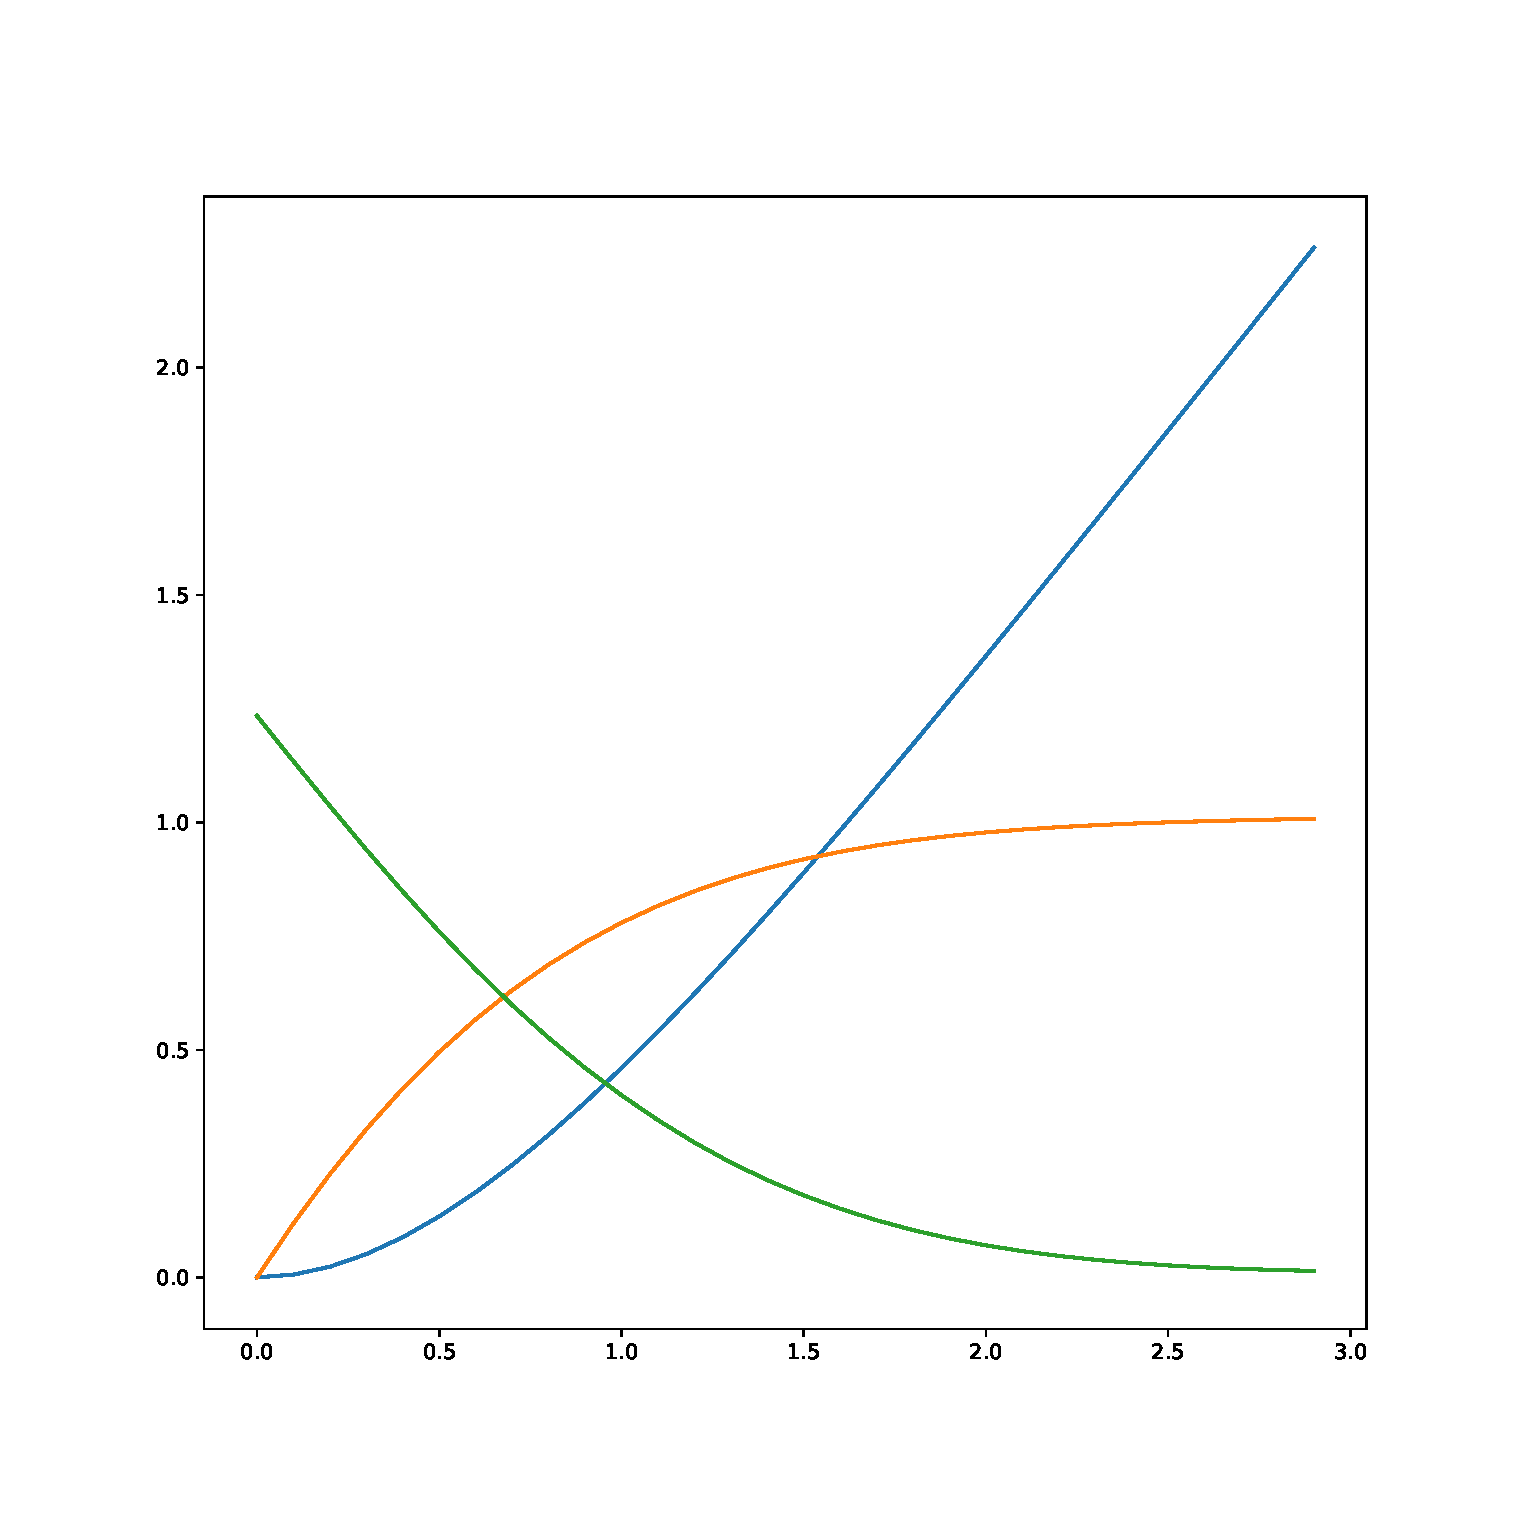
\includegraphics[width=0.4\linewidth]{figures/stagnation_functions}
    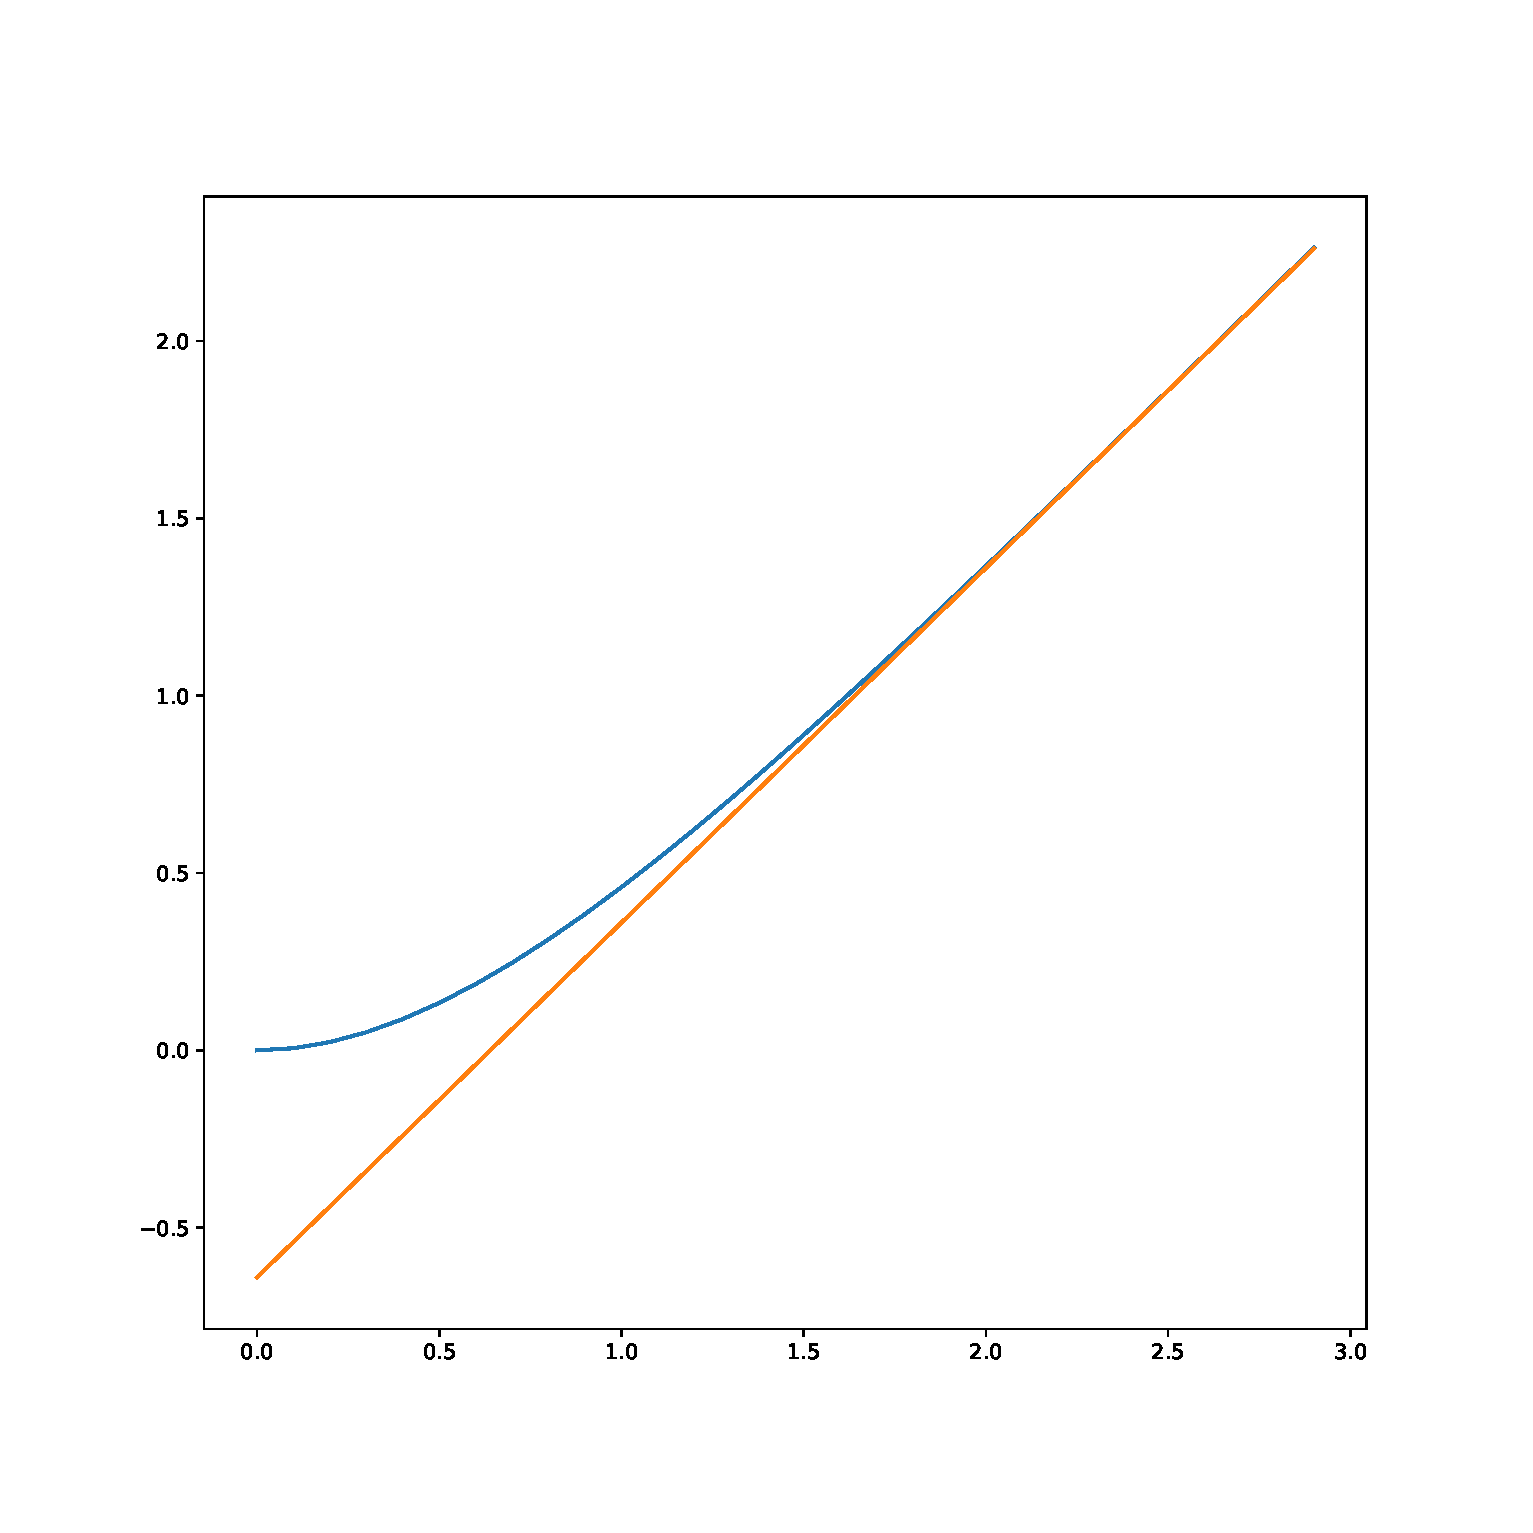
\includegraphics[width=0.4\linewidth]{figures/stagnation_function_disp}
  \caption{\label{fig:stagnation_functions}}
\end{figure}


In Figure \ref{fig:stagnation_functions} left, the function $g$ and
its first and second derivatives are plotted. With these, it is easy
to plot the resulting streamlines, Figure
\ref{fig:stagnation_streamlines} right. In the latter, the potential
streamlines are shown in the left. It is apparent how the flow is
``moved upwards'' due to viscous effects near the wall. This
displacement is readily quanfified by the asympotic behavour of $g$,
as shown in Figure \ref{fig:stagnation_functions} left. A reasonable
approximation is
\[
g(y) \approx -0.64 + y .
\]
This provides an estimate of the boundary layer thickness as given
by
\[
\delta = 0.64 \ell =  0.64 \sqrt{\nu/B} ,
\]
which then increases as the root square of $\nu$, and decreases as,
basically, the root square of the velocity far away from the wall
(through $B$).

To get some numbers, if air approaches a \SI{10}{\centi\meter}
diameter cylinder at $u_0=\SI{10}{\meter\per\second}$, then
$B = 4u_0/D =\SI{400}{\per\second}$ (there is a factor of $4$
involved, see \cite{white1991viscous} \S 7.3 ). With
$\nu\approx\SI{1.5e-5}{\meter\squared\per\second}$, we get
$\delta = \SI{0.12}{\milli\meter}$, a very thin layer. The thickness
of the layer can be defined in other ways, for example as the distance
at which $f'(y) \approx 0.99 $ (so that the value of $u_x = B x f'$ is
$99\%$ its potential solution value, $B x$.) This yields
$\approx 2.4 \ell$, which is about $3.7$ times larger than
$\delta$. Still, only approximately $ \SI{0.44}{\milli\meter}$, beyond
which the effect of the wall is quite neglibible.

This fact is a blessing, since it restores our faith in
potential-based solutions: many flows look potential flows when viewed
at some distance from obstacles (indeed, away from any region that may
generate vorticity and involve shear, such as jets, wakes \ldots). It
also solves d'Alembert's paradox, since the velocity field can still
comply with the no-slip boundary condition and exert drag forces on
obstacles (in general, they will be due both to pressure and to wall
shear stress). It is also a curse mathematically: the details of a
proper matching between it the layer and the flow around it must be
worked out carefully. Also computationally, the fact that the boundary
layer is so thin compared with other dimensions of the problem leads
to prohibitively large simulation meshes, or the necessity to refine
the meshes close to surfaces. The latter fact favours methods such as
the finite element method, or the finite volume method, in which
refinement is easier, over other ones like finite differences.

The pressure was partly known already, $p=-(B^2/2) x^2 + h(y)$. The other
Navier-Stokes equation, which we have still not used, reads
\[
B f B f'  =  - \frac{\partial p}{\partial y} -
\nu B  f'' .
\]
This means
\[
h' = - B^2 f f' - \nu B f'' ,
\]
which may be easily integrated :
\[
h = -B^2 \frac12 f^2  - \nu B f' .
\]
So, finally:
\[
p = -\frac{1}{2} \left[
  (B x)^2 +
  (B f)^2
  \right]  - \nu B f' =
 -\frac{1}{2} \left[
  (u_x / f' )^2 +
  u_y^2
  \right]  - \nu B f' ,
 \]
 where the last equality shows that the pressure is not so different
 from the potential solution, Eq. \ref{eq:p_stag_pot}.
%
 Notice it is not $u_X$ which features, but rather $u_x/f'$, which
 does tend to the $u_x$ away from the wall. An additional, viscous
 term appears, which makes the pressure have a constant offset
 $-\nu B$ with respect to its potential counterpart, as we move
 away from the wall.

 Pressures are also included in Fig.
 \ref{fig:stagnation_streamlines}. To make a more quantitative
 comparison, isobars are plotted in
 Fig. \ref{fig:stagnation_pressures}. It is interesting that viscosity
 causes pressure to be ``pushed'' against the wall, flattening the
 isobars (and, interestingly, making them not normal to the
 wall). While, far away from the wall, they approach the same circular
 shape, but with a constant offset. In these figures, pressures are
 plotted in their reduced form. It is easy to check that the pressure
 scale is given by $B \nu$ (units of velocity squared --- remember this
 is the dynamic pressure).

\begin{figure}
  \centering
  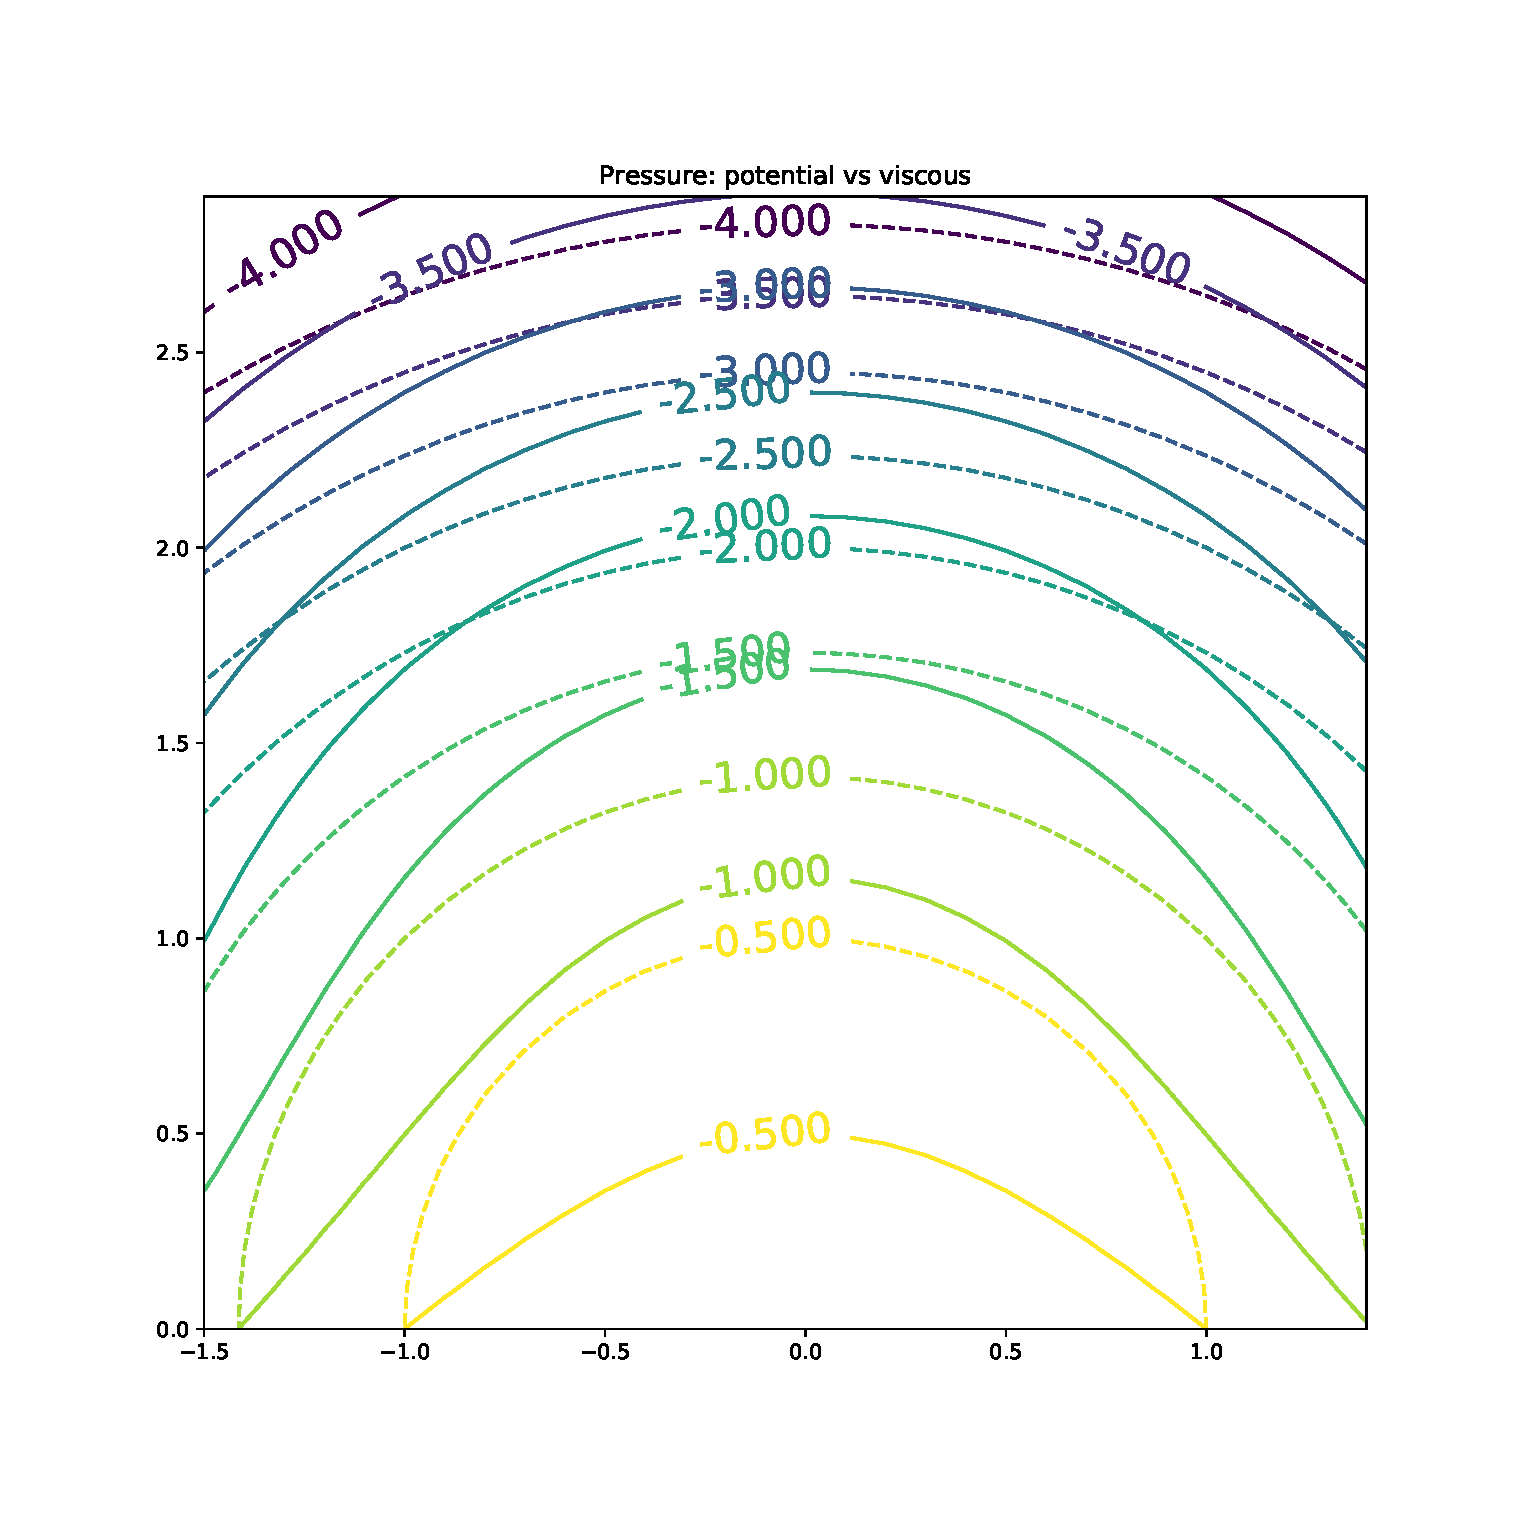
\includegraphics[width=0.6\linewidth]{figures/stagnation_potential_viscous_pressures}
  \caption{\label{fig:stagnation_pressures}}
\end{figure}

Another interesting feature of the flow is its vorticity, which is
readily computed from
\[
\omega_z =
\frac{\partial u_y}{\partial x} -
\frac{\partial u_x}{\partial y} =
0 - B x f''(y)  = - B x^* g''(y^*) .
\]
Hence the wall is seen to induce vorticity close to it, with a sign change
on both sides on the $x=0$ symmetry plane. The shear stress is given by a
similar expression,
\[
\tau_{xy}= \mu
\left(
\frac{\partial u_y}{\partial x} +
\frac{\partial u_x}{\partial y}
\right)
 =  \mu B  x f''(y)  = \mu B x^* g''(y^*) .
 \]

 In particular, the wall stress is
 \[
 \tau_\mathrm{w}:=\tau_{xy}(y=0) = \mu B x^* g''(0)
 \approx 1.234 \mu B x^*
 \]

 The (horizontal) skin friction coefficient may be defined, for this problem,
 as
 \[
 C_\mathrm{f} := \frac{2 \tau_\mathrm{w} }{ \rho (B x)^2 } .
 \]
 The denominator features the horizontal velocity away from the wall,
 $B x$. Then,
 \[
 C_\mathrm{f} := \frac{2 \sqrt{B\nu}  g''(0) }{ B x } =:
 \frac{2   g''(0) }{\sqrt{ \mathrm{Re}_x} } ,
 \]
 where the local Reynolds number is defined as
 \[
 \mathrm{Re}_x = \frac{(Bx) x}{\nu} .
 \]
 I.e. a Reynolds number where the typical velocity is the horizontal
 velocity far from the wall, $Bx$, and the distance is that to the
 impact point, $x$. A dependence of the friction coefficient with the
 inverse square root of a local Reynolds number is a common feature of
 laminar boundary layers.
 


\chapter{Turbulence}
